\documentclass[conference]{IEEEtran}
\IEEEoverridecommandlockouts
% The preceding line is only needed to identify funding in the first footnote. If that is unneeded, please comment it out.
\usepackage{cite}
\usepackage{amsmath,amssymb,amsfonts}
\usepackage{algorithmic}
\usepackage{graphicx}
\usepackage{textcomp}
\usepackage{xcolor}
\usepackage{float}
\usepackage{wrapfig}
\usepackage{hyperref}
\usepackage{atbegshi}
\usepackage{fancyhdr}
\def\BibTeX{{\rm B\kern-.05em{\sc i\kern-.025em b}\kern-.08em
    T\kern-.1667em\lower.7ex\hbox{E}\kern-.125emX}}
\begin{document}

\title{Clean Out}

\author{\IEEEauthorblockN{1\textsuperscript{st} Kishan Sakdasariya}
\IEEEauthorblockA{
\textit{DAIICT}\\
Gandhinagar, India \\
20170158@daiict.ac.in}
\and
\IEEEauthorblockN{2\textsuperscript{nd} Bhavik Chhotala}
\IEEEauthorblockA{
\textit{DAIICT}\\
Gandhinagar, India \\
20170217@daiict.ac.in}
\and
\IEEEauthorblockN{3\textsuperscript{rd} Darshit Nasit}
\IEEEauthorblockA{
\textit{DAIICT}\\
Gandhinagar, India \\
20170412@daiict.ac.in}
}
\maketitle

\fancypagestyle{footer}{\fancyhf{}\renewcommand{\headrulewidth}{0pt}\fancyfoot[R]{Prof. Jayprakash Lalchandani(jayprakash\_lalchandani@daiict.ac.in), DAIICT, Gandhinagar, Gujarat, INDIA}}
\pagestyle{fancy} % or whatever



\begin{abstract}
Clean out is web-application where user can provide and book cleaning services, shopkeeper can sell cleaning products. In this document whole process of developing the app is given. Starting with features and functions, UML diagrams, implementation and testing, at the end the paper there is discussion about future plan/works and conclusion. \\

Keywords - Cleaning service, E-commerce, MVC design pattern, MERN stack\\

\end{abstract}





\section{Introduction}
\thispagestyle{footer}
Almost everyone needs cleaning services for office, shop, house, garden, marriage/party hall, etc. There are many workers who provides these services. So, clean out is connecting these two groups on one platform. For cleaning services many products like brooms, soap, hand gloves, washing liquid/powder, etc. Clean out also provides features where shopkeeper can sell cleaning products. So,user can book service and order cleaning items needed for service from same platform. Here shopkeeper can also have workers providing services under them.\\ 

Basically there are five type of users:
\begin{enumerate}
    \item Customer
    \item Worker
    \item Shopkeeper
    \item Admin
    \item Coadmin \\
\end{enumerate}

User can register themselves into clean out and order service. Each user must have unique contact number as all the notifications would be sent to that number. Worker and Shopkeeper are service providers. They can add services of their own, but only workers can go to customer and provide service. To achieve this goal shopkeeper must have to add some workers under his/her shop. For registration service providers needs to upload their ID proof for verification and worker has to upload profile picture. Also there is OTP verification feature so that only booked worker is allowed to provide the service. User or service provider can cancel ordered service. After service user can give feedback to the worker.\\





\section{Features and User stories}
\subsection{Customer}
\begin{enumerate}
    \item Registration : As a customer I want registration form so that I can register myself.
    \item Update : As a customer I want an update profile feature so that I can update details.
    \item Delete : As a customer I want an delete profile feature so that I can delete my profile.
    \item Login : As a customer I want login so that I can login to the website.
    \item Logout : As a customer I want logout feature so that I can logout from the website.
    
    \item Get services : As a customer I want a page where I can see all services in pagination form.
    \item Get items : As a customer I want a page where I can see all items in pagination form.
    
    \item Search service by category : As a customer I want a selection bar so that I can search services by service category.
    \item Search service by subcategory : As a customer I want a selection bar so that I can search services by service subcategory.
    \item Sort services/items by price : As a customer I would like to have a sort option so that I can sort services/items by price.
    \item Sort services/items by rating : As a customer I would like to have a sort option so that I can sort services/items by rating value.
    \item Sort services/items by popularity : As a customer I would like to have a sort option so that I can sort services popularity.
    \item View service : As a customer I want profile of service so that I can get description and rating.
    \item View price : As a customer I want to add my requirement into profile of service so that I can get the price.
    \item Book service : As a customer I want features so that I can book service.
    \item Cancel service : As a customer I want features so that I can cancel booked service.
    
    \item Search item by name : As a customer I want a search bar so that I can search items by name.
    \item View item : As a customer I want profile of cleaning item so that I can get description and rating.
    \item Add item to cart : As a customer I want a cart in which I can store cleaning items.
    \item Remove item from cart : As a customer I want a cart from which I can remove cleaning items.
    \item Place order : As a customer I want features so that I can place order.
    \item Cancel order : As a customer I want features so that I can cancel order.
    
    \item Give feedback : As a customer I want a review (written) panel so that I can write review for both cleaning item and services.
    \item Get notifications : As a customer I would like to get notifications about service order and cleaning item order after exactly one month of placing order.
    \item Buy again : As a customer I want to have the buy again option so that I can buy again previous ordered cleaning items and services.
\end{enumerate}
    
\subsection{Worker}
\begin{enumerate}
    \item Update profile : As a worker I should be able to update profile and when I update profile I should become non verified.
    \item Add service : As a worker I should be able to add service.
    \item Update service : As a worker I should be able to update service.
    \item Delete service : As a worker I should be able to delete service.
    \item Get service order : As a worker I want a feature so that I can get service details and customer’s address.
    \item Get/Verify OTP : As a worker I want get OTP and verify OTP feature so that I can verify myself.
    \item Cancel service order : As a worker I should be able to cancel placed service.
    \item See ratings : As a worker I should be able to see the ratings/review given to me by customers so that I can improve my services.
    \item Accept shopkeeper request : As a worker I should be able to accept request from shopkeeper to become the shopkeeper’s worker (shopkeeper based worker).
    \item Shopkeeper based worker : As a worker when I become shopkeeper’s worker, I should not be able to edit any service details of shopkeeper and I should not have any services.
    \item Work done : As a worker I want a feature so that I can notify the system that I have completed service.
    \item Camera : As a worker I want camera feature so that I can take pictures of myself and ID proofs to register myself.
    \item Preferred locations : As a worker I want preferred location field so that I can go to only my preferred locations to provide service.
    \item Requested orders : As a worker I want a page where I can see all the item orders and service orders sorted by date in pagination format.
\end{enumerate}
    
\subsection{Shopkeeper}
\begin{enumerate}
    \item Update profile : As a shopkeeper I should be able to update profile and when I update profile I should become non verified.
    \item Add service : As a shopkeeper I should be able to add service.
    \item Update service : As a shopkeeper I should be able to update service.
    \item Delete service : As a shopkeeper I should be able to delete service.
    \item Add item : As a shopkeeper I should be able to add item.
    \item Update item : As a shopkeeper I should be able to update item.
    \item Delete item : As a shopkeeper I should be able to delete item.
    \item Add worker : As a shopkeeper I should be able to send request to worker to work under me.
    \item Delete worker : As a shopkeeper I should be able to delete worker.
    \item Get service order/item order
    \item Cancel service order : As a shopkeeper I should able to cancel placed service if worker is not available.
    \item Cancel item order : As a shopkeeper I should able to cancel item order.
    \item Requested orders : As a shopkeeper I want a page where I can see all the item orders and service orders sorted by date in pagination format.
\end{enumerate}

\subsection{Admin}
\begin{enumerate}
    \item Add Coadmin : As an admin I want a feature so that I can make a user Co-admin.
    \item Remove Coadmin : As an admin I want a feature so that I can make a Co-admin user.
\end{enumerate}
    
\subsection{Admin/Coadmin}
\begin{enumerate}
    \item Any user registration : As a admin/coadmin I should be able to add any type of user.
    \item Any user update : As a admin/coadmin I should be able to update any type of user.
    \item Any user delete : As a admin/coadmin I should be able to delete any type of user.
    \item Add service/item for worker/shopkeeper : As a admin/coadmin I should be able to add service or item for shopkeeper or worker.
    \item Update service/item for worker/shopkeeper : As a admin/coadmin I should be able to update service or item.
    \item Delete service/item for worker/shopkeeper : As a admin/coadmin I should be able to delete service or item.
    \item See statistics : As a admin/coadmin I should be able to see statistics of the website.
    \item Verify worker/shopkeeper : As a admin/coadmin I should be able to verify worker and shopkeeper based on the proofs they provided.
    \item Search user : As an admin/coadmin I want a search bar so that I can search users by name, contact number and pincode.
\end{enumerate}





\vspace{1cm}
\section{MVC Pattern}
\begin{figure}[H]
    \centering
    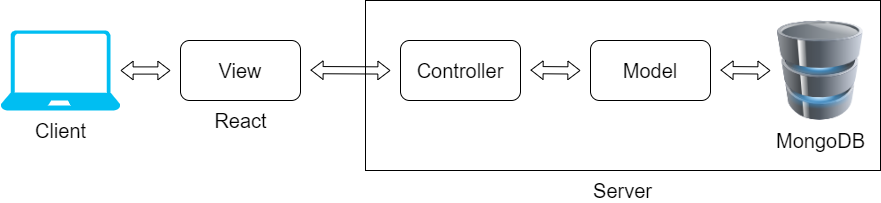
\includegraphics[width=8cm]{MVC.png}
    \caption{MVC design pattern}
    \label{fig:mvc}
\end{figure}

\begin{minipage}{3cm}
    \begin{figure}[H]
        \centering
        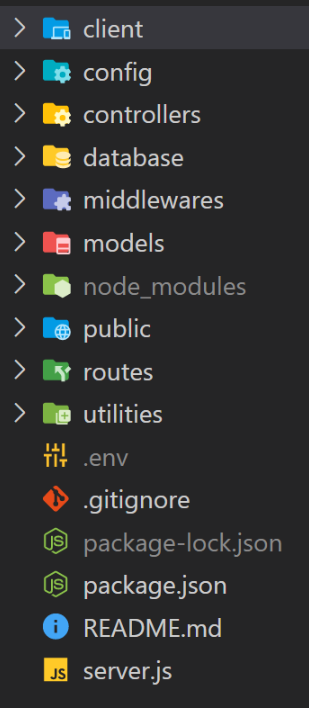
\includegraphics[width=3cm]{FolderStructure.png}
        \caption{Folder Structure}
        \label{fig:folderStructure}
    \end{figure}
\end{minipage} \
\begin{minipage}{5.3cm}
    In this project we have used MVC design pattern. M stands for Model which interacts with database and save/update/delete data. V stands for View which is UI and C stands for controller which takes request and generate output according to request. As you can see from figure \ref{fig:mvc} client is interacting with react directly and react sends request to backend according to user input. In the figure \ref{fig:folderStructure} we have shown the folder structure of the application. We have mapped Model to our models folder. Each file in the models folder act as mongodb model which directly interacts with mongodb. View is mapped to client folder, which contains react js code,
\end{minipage}%

\vspace{-0.2cm}
\hspace{3.14cm} which is rendered at the client browser. And Controller is mapped to controllers folder, where each file in controller act as endpoint for a specific resource.








\vspace{0.5cm}
\section{Tools and Technologies}
\begin{enumerate}
    \item MongoDB : The database we have used in the application
    \item Express : A web server allowing uss to host application online
    \item React JS : Library to implement frontend
    \item Node JS : Javascript engine to run javascript application locally and to implement backend
    \item Visual Studio Code : IDE to write code
    \item MongoDB CLI : To interact with mongodb
    \item MongoDB Compass : For testing purpose, it shows all data available in mongodb
    \item Postman : For backend API testing
    \item Figma : To make UI design
    \item Google Chrome
    \item Mozilla Firefox
    \item Opera
\end{enumerate}








\newpage
\section{Design (UML Diagrams)}

\vspace{1cm}
\subsection{Activity Diagrams}
\begin{figure}[H]
    \centering
    \includegraphics[width=7.5cm]{activity-1.jpg}
    \caption{Search, book service and OTP verification}
    \label{fig:activity1}
\end{figure}
\begin{figure}[H]
    \centering
    \includegraphics[width=8cm]{activity-4.jpg}
    \caption{View/Update Profile}
    \label{fig:activity4}
\end{figure}
\begin{figure}[H]
    \centering
    \includegraphics[width=8cm]{activity-3.jpg}
    \caption{Login and Registration}
    \label{fig:activity3}
\end{figure}
\begin{figure}[H]
    \centering
    \includegraphics[width=8cm]{activity-2.jpg}
    \caption{Shopping cleaning items}
    \label{fig:activity2}
\end{figure}



\subsection{Sequence Diagram}
\begin{figure}[H]
    \centering
    \includegraphics[width=8cm]{seq-1.jpg}
    \caption{User registration}
    \label{fig:seq1}
\end{figure}
\begin{figure}[H]
    \centering
    \includegraphics[width=8cm]{seq-2.jpg}
    \caption{Add item in cart}
    \label{fig:seq2}
\end{figure}
\begin{figure}[H]
    \centering
    \includegraphics[width=8cm]{seq-3.jpg}
    \caption{Place Order}
    \label{fig:seq3}
\end{figure}
\begin{figure}[H]
    \centering
    \includegraphics[width=8cm]{seq-4.jpg}
    \caption{Get OTP}
    \label{fig:seq4}
\end{figure}
\begin{figure}[H]
    \centering
    \includegraphics[width=8cm]{seq-5.jpg}
    \caption{Verify OTP}
    \label{fig:seq5}
\end{figure}
\begin{figure}[H]
    \centering
    \includegraphics[width=8cm]{seq-6.jpg}
    \caption{Book service}
    \label{fig:seq6}
\end{figure}



\subsection{Use Case Diagram}
\begin{figure}[H]
    \centering
    \includegraphics[width=9cm]{usecase.jpg}
    \caption{Use case Diagram}
    \label{fig:usecase}
\end{figure}






\newpage
\subsection{Class Diagram}
\begin{figure}[H]
    \centering
    \includegraphics[width=9cm]{class.jpg}
    \caption{Class Diagram}
    \label{fig:class}
\end{figure}




\vspace{2cm}
\subsection{UI Design}
\begin{figure}[H]
    \centering
    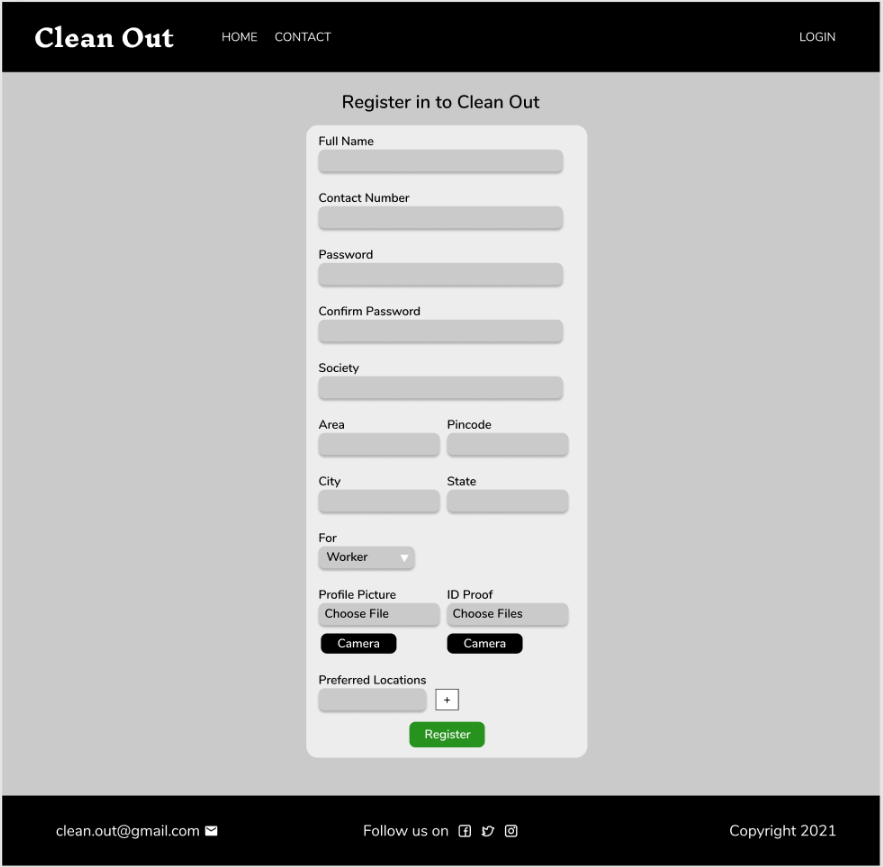
\includegraphics[width=8cm]{Register worker.png}
    \caption{Register worker}
    \label{fig:registerWorker}
\end{figure}
\begin{figure}[H]
    \centering
    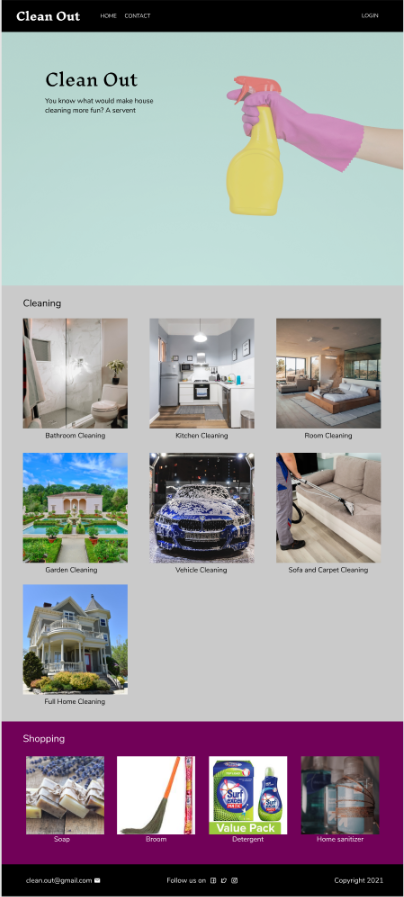
\includegraphics[width=8cm]{Home.png}
    \caption{Home page}
    \label{fig:home}
\end{figure}
\begin{figure}[H]
    \centering
    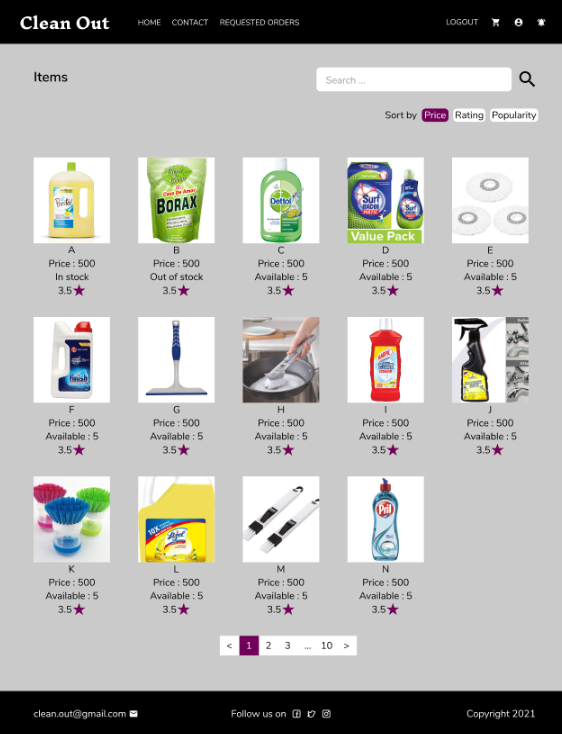
\includegraphics[width=8cm]{Item store.png}
    \caption{Item store}
    \label{fig:itemStore}
\end{figure}
\begin{figure}[H]
    \centering
    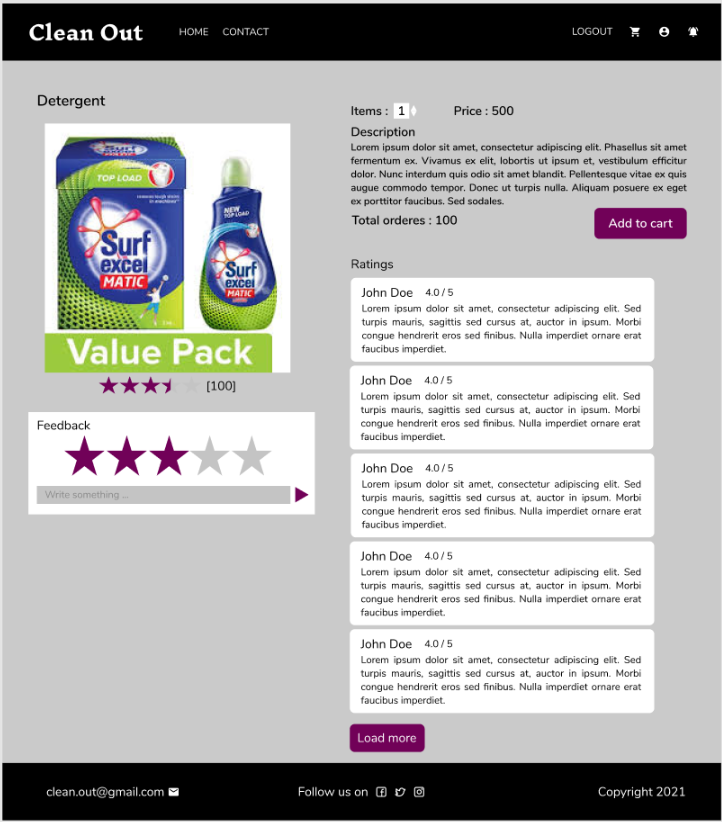
\includegraphics[width=8cm]{View Item.png}
    \caption{View item}
    \label{fig:viewItem}
\end{figure}
\begin{figure}[H]
    \centering
    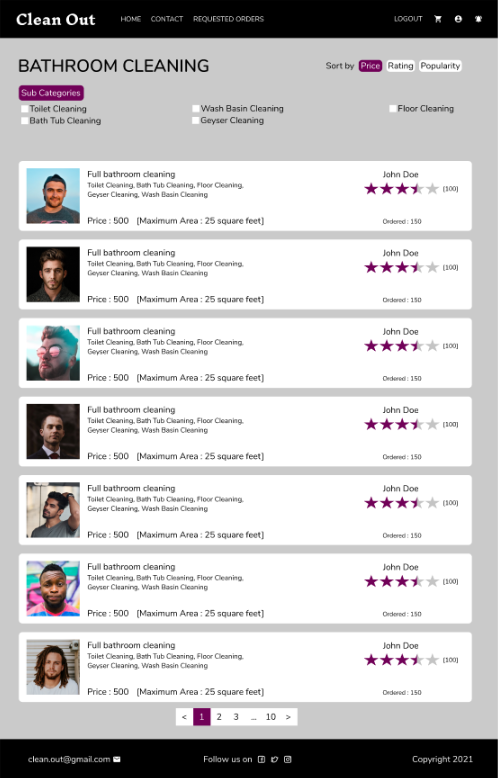
\includegraphics[width=7.5cm]{Service store.png}
    \caption{Service store}
    \label{fig:serviceStore}
\end{figure}
\begin{figure}[H]
    \centering
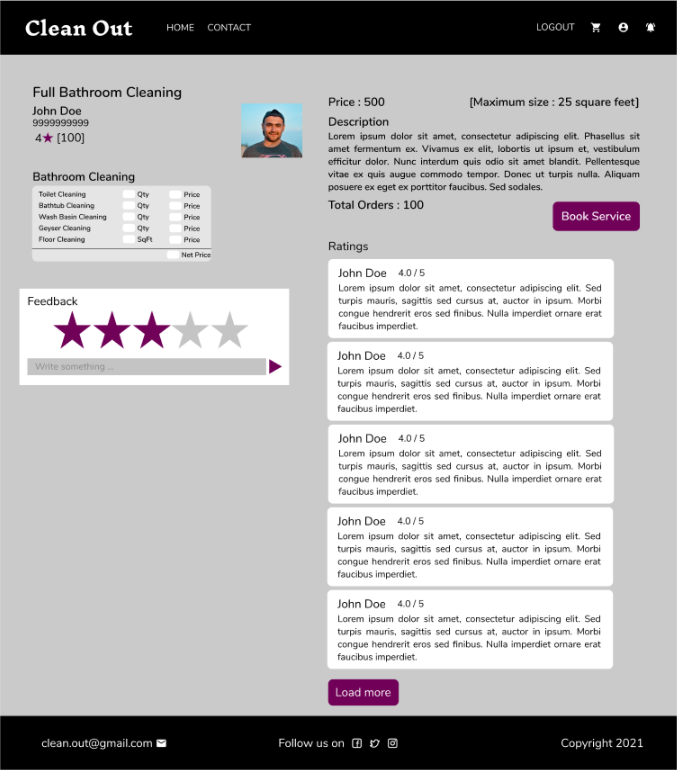
\includegraphics[width=8cm]{View Worker Service.png}
    \caption{View worker service}
    \label{fig:viewWorkerService}
\end{figure}
\begin{figure}[H]
    \centering
    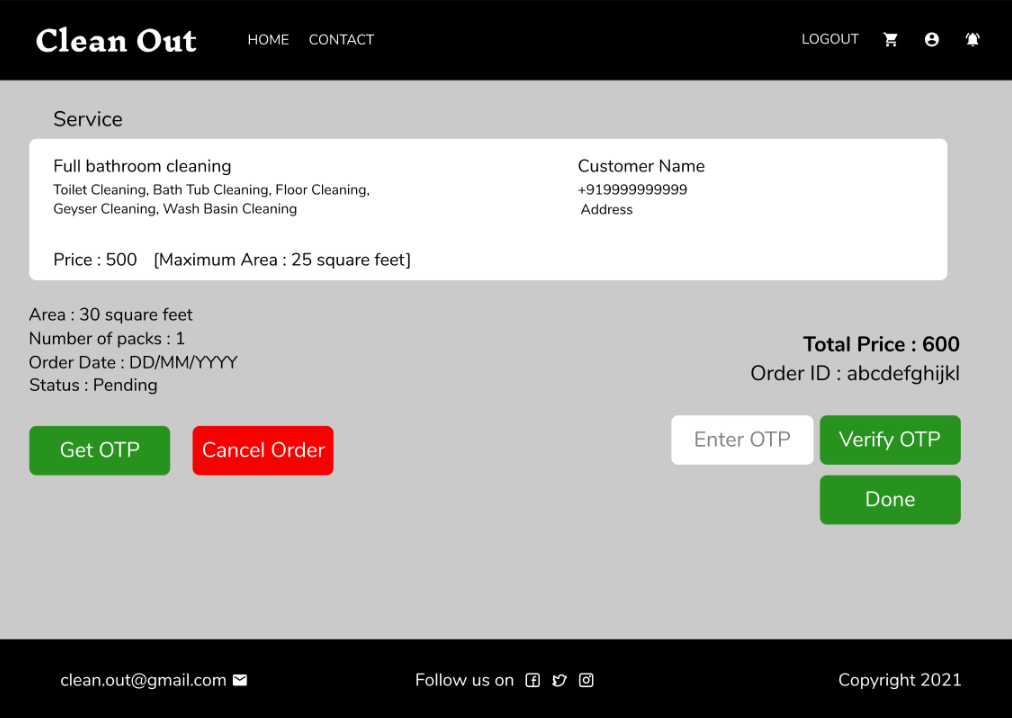
\includegraphics[width=7.5cm]{View worker service order.png}
    \caption{Worker service oreder}
    \label{fig:viewWorkerServiceOrder}
\end{figure}








\vspace{1cm}
\section{Testing}
Testing is a crucial part of any application. So to begin with we first tried unit testing. We performed unit testing on small scale components like buttons, links and forms when and where they should be enabled and functionalities of the same with validations. 

\begin{itemize}
    \item Given below is register form which successfully passed all the test cases and similarly other forms.
    \begin{figure}[H]
        \centering
        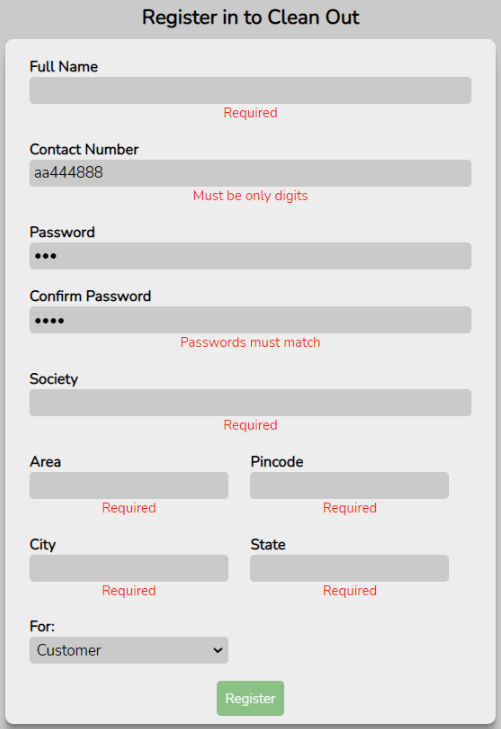
\includegraphics[width=7.5cm]{Testing register.png}
        \caption{Testing register form}
        \label{fig:testRegister}
    \end{figure}
     In each form if field is contact number then input must have all digits and length must be exact 10. If field is pincode then all digits and length of 6. If confirm password field then it must match with password field. All forms have passed in this test.
    
    \vspace{0.5cm}
    \item In register form when user try to register with contact number which is already registered then application will not allow that.
    \begin{figure}[H]
        \centering
        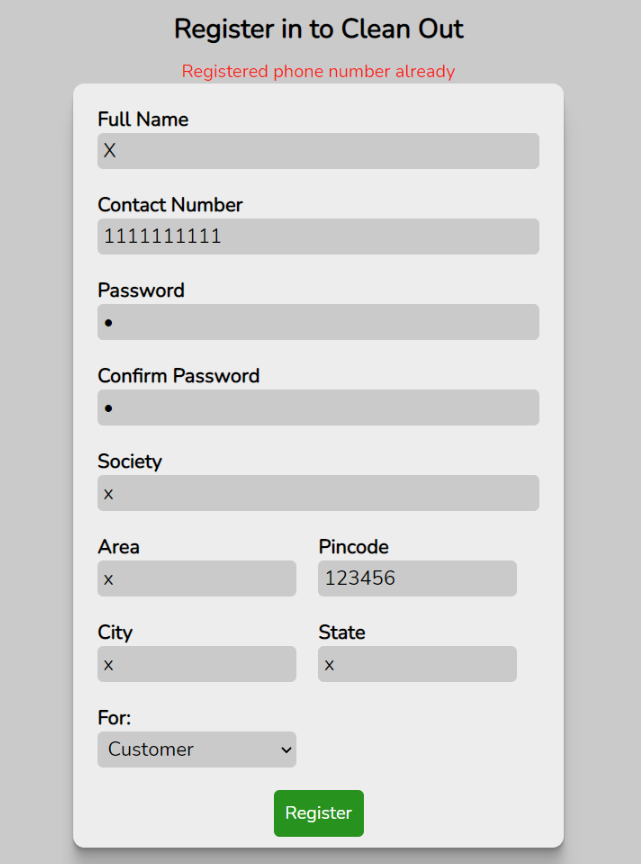
\includegraphics[width=8cm]{Testing register with same phone.png}
        \caption{Testing register with same contact number}
        \label{fig:testRegisterWithSamePhone}
    \end{figure}
    
    \item The other main unit test was to check whether selection of subcategories in service store are working properly or not and below are the results.
    \begin{figure}[H]
        \centering
        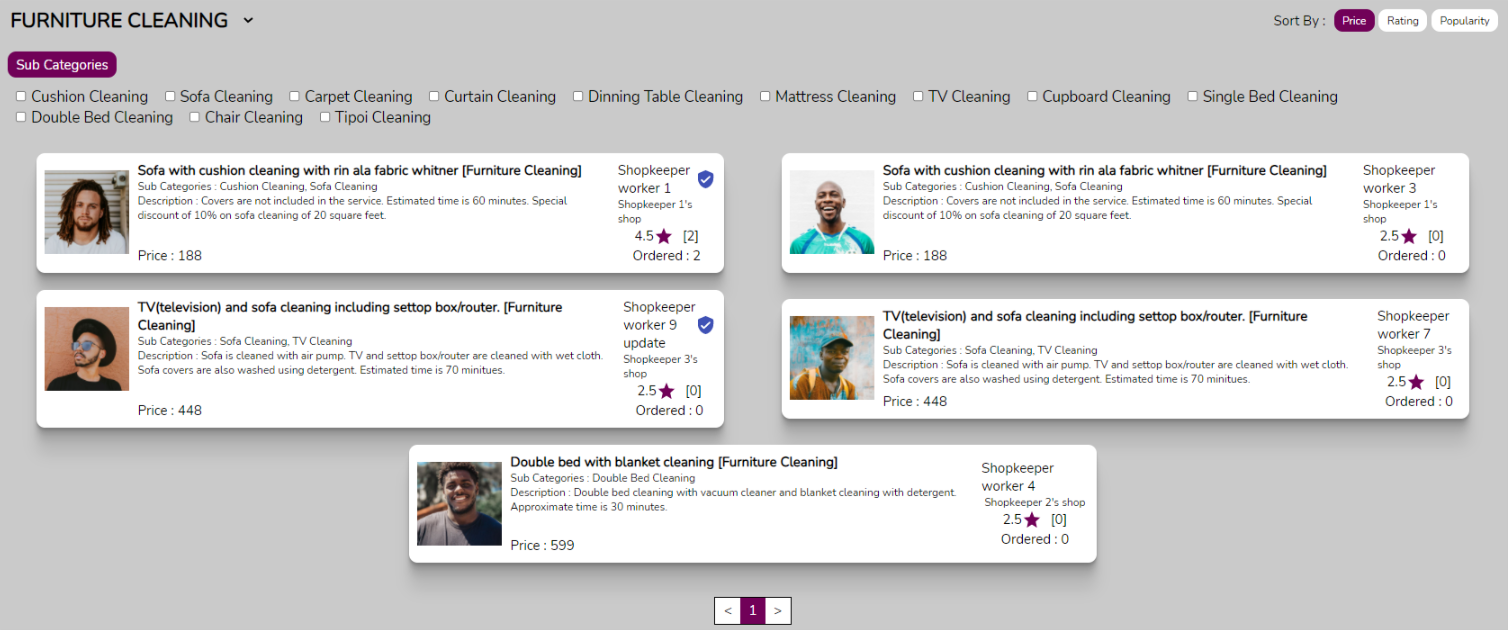
\includegraphics[width=8cm]{Testing service category before.png}
        \caption{Testing service category before any input}
        \label{fig:testServiceCategoryBefore}
    \end{figure}
    \begin{figure}[H]
        \centering
        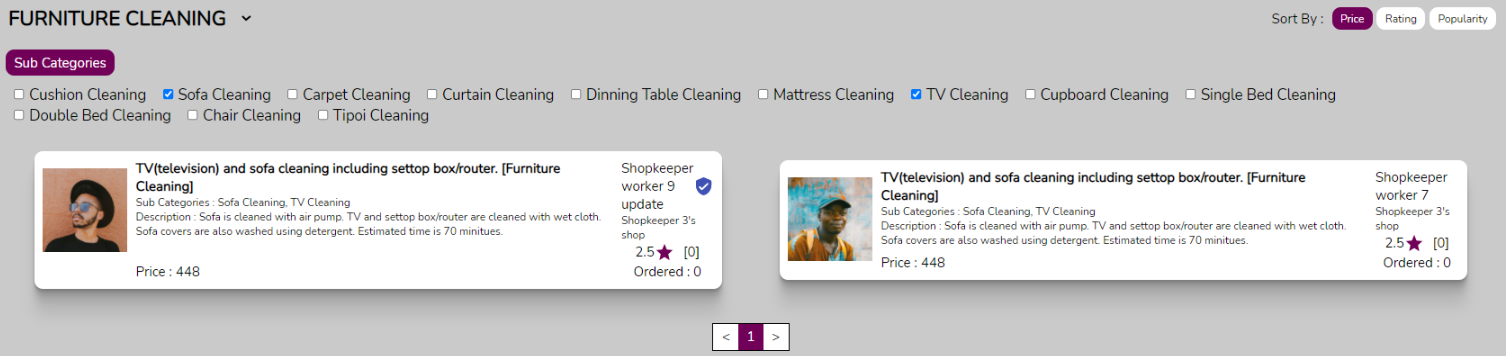
\includegraphics[width=8cm]{Testing service category after.png}
        \caption{Testing service category after selecting some fields}
        \label{fig:testServiceCategoryAfter}
    \end{figure}
    
    \item Another thing we tested is when shopkeeper sent request to worker it shows in the notification bar. Here we also tested that if the request is already sent once then shopkeeper cannot sent request again and if worker is already under some other shopkeeper then shopkeeper cannot sent request.
    \begin{figure}[H]
        \centering
        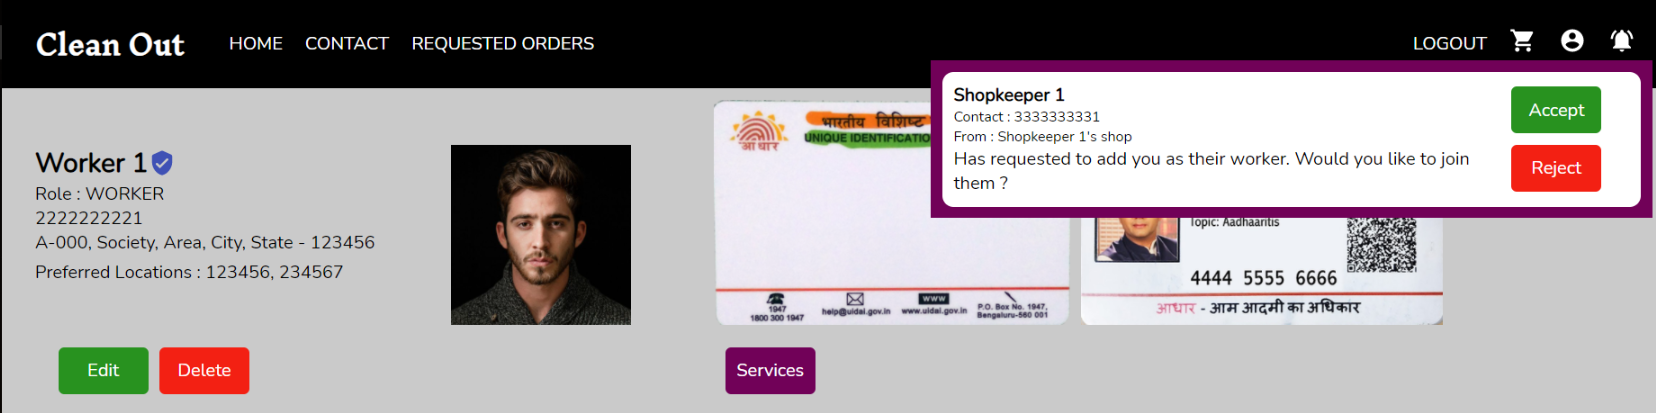
\includegraphics[width=8cm]{Testing shopkeeper request.png}
        \caption{Testing shopkeeper request sent to worker}
        \label{fig:testShopkeeperRequest}
    \end{figure}
    
    \item Then we tested the notification part also. When the user book service or place order or cancel order appropriate user/worker/shopkeeper gets notification regarding the same. Also we have used cron jobs in application to send remainders after one month of placing any type of order. So all those were also running successfully. Right now we do not have any external service for sending notification via SMS, so for simplicity we just logging message in the console. Below is the result when customer book service of a shopkeeper. In that case notification is sent to customer itself then shopkeeper and the worker of the shopkeeper that selected by customer.
    \begin{figure}[H]
        \centering
        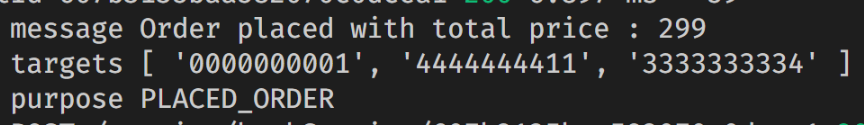
\includegraphics[width=8cm]{Testing notifications.png}
        \caption{Testing notification on booking service}
        \label{fig:testNotification}
    \end{figure}
    
    \item With above we tested if the application is allowing further operation whether OTP entered is correct or not. There are two cases where we need actions based on OTP. First one is forgot password use case and second is verify correct worker has come to provide service. In both scenario our application passed test case. Below is figures for reset password use case.
    \begin{figure}[H]
        \centering
        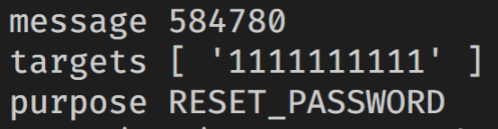
\includegraphics[width=8cm]{Testing reset otp get.png}
        \caption{Testing sending reset password OTP to user}
        \label{fig:testResetPasswordGet}
    \end{figure}
    \begin{figure}[H]
        \centering
        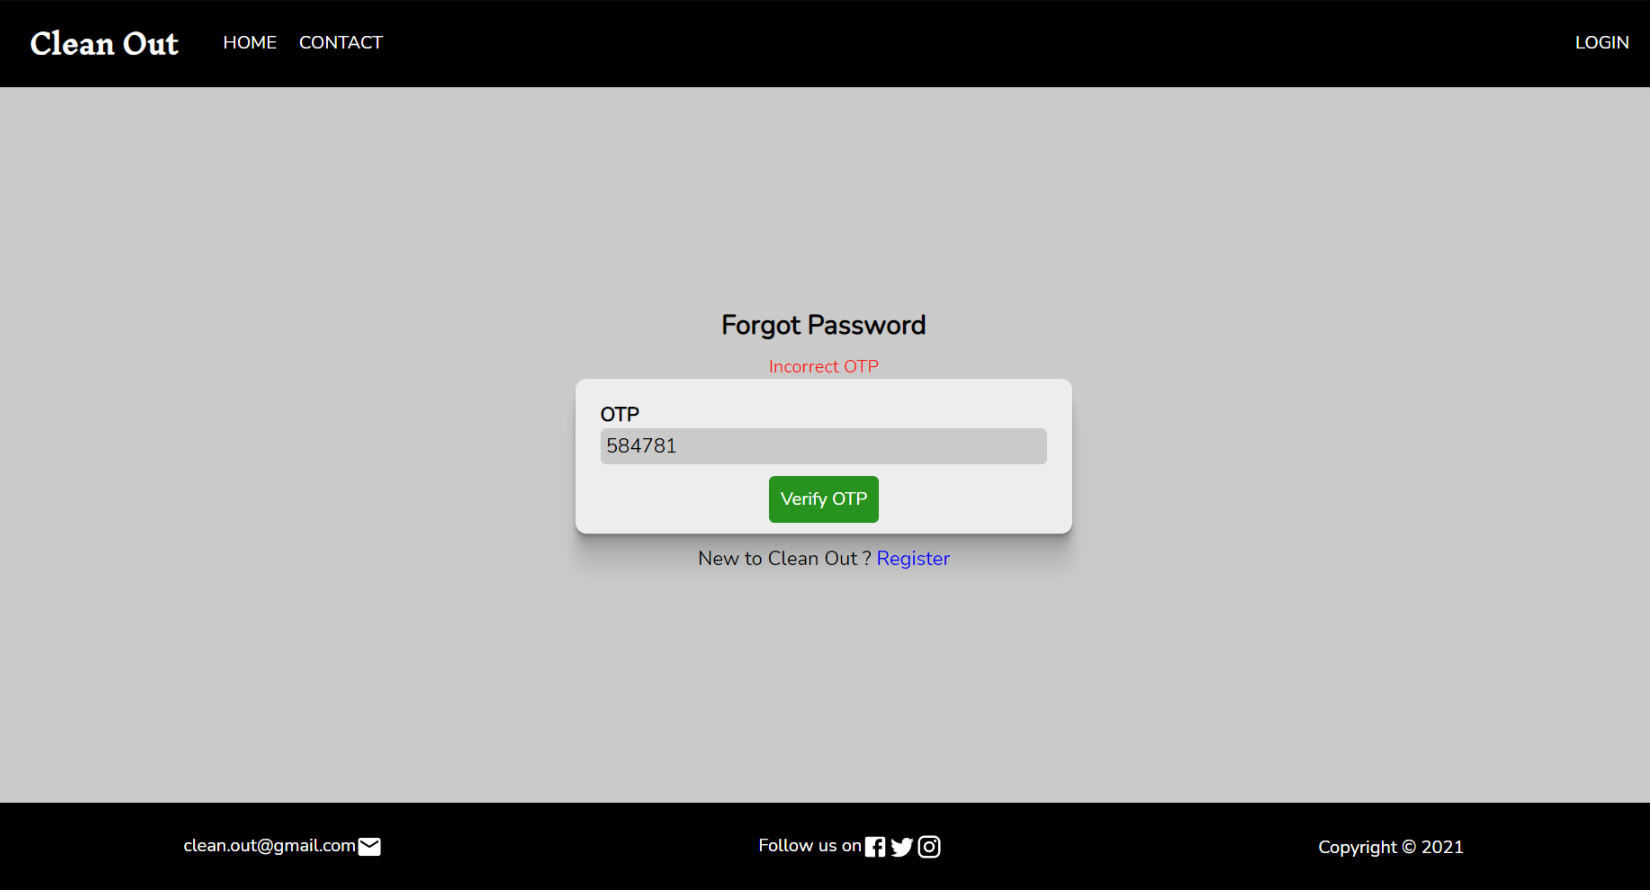
\includegraphics[width=8cm]{Testing reset otp verify.png}
        \caption{Testing validating reset password OTP}
        \label{fig:testResetPasswordVerify}
    \end{figure}
    
    \item In the application we filter services and show to customer based on the address pincode of the logged in user. But if customer is not logged in then we manually ask pincode of their area and based on that pincode we show the services.
    \begin{figure}[H]
        \centering
        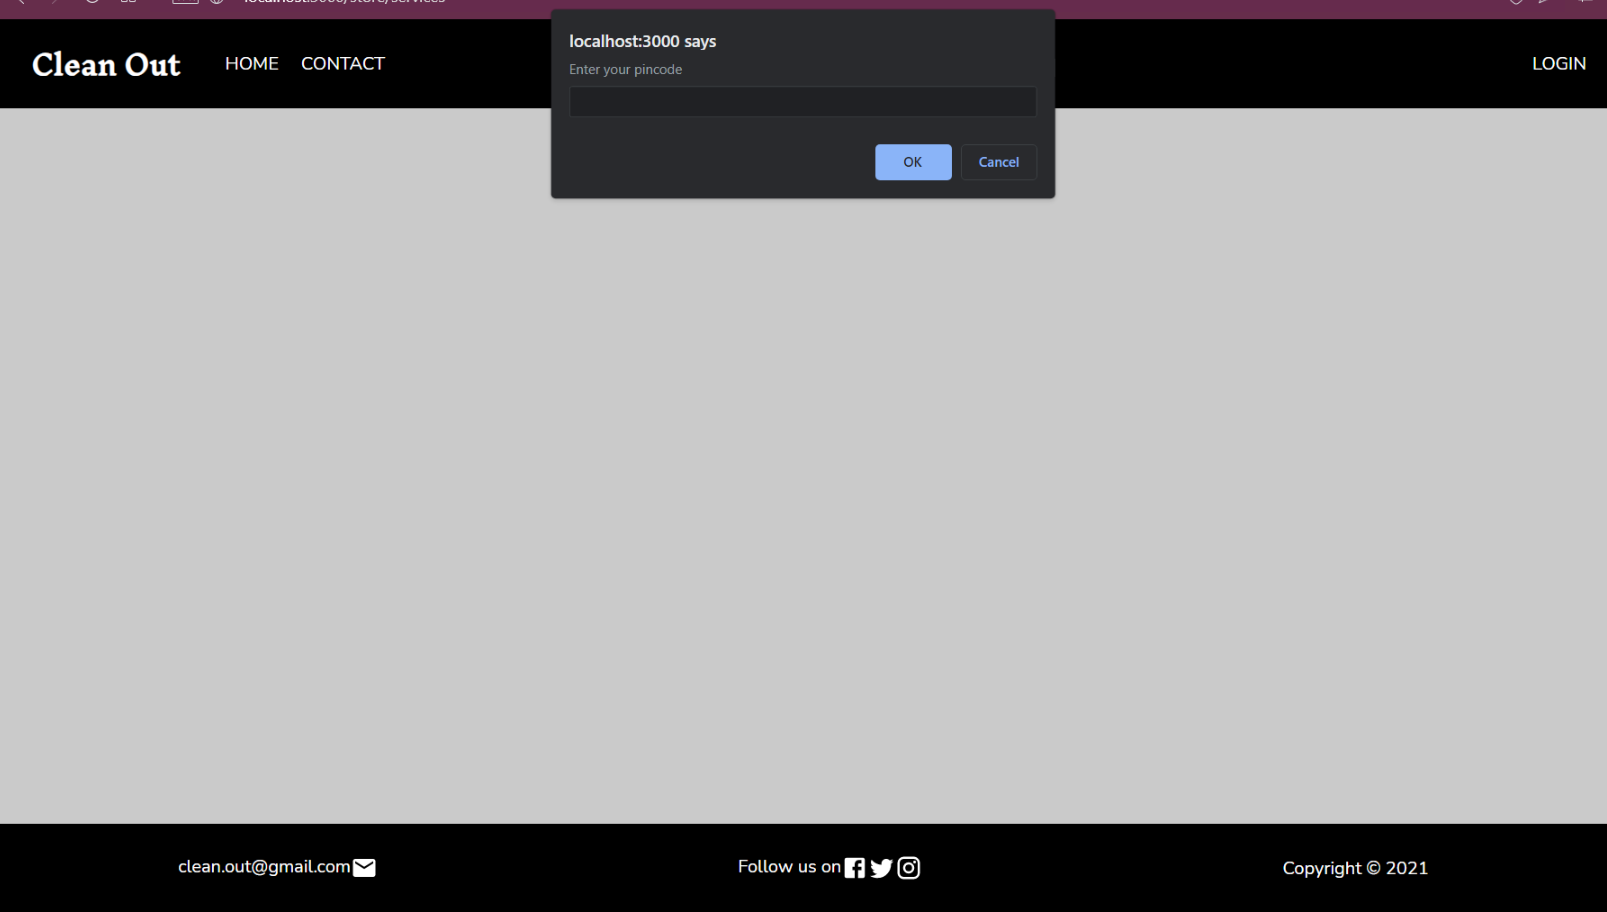
\includegraphics[width=8cm]{Testing pincode 1.png}
        \caption{Testing pincode propmt if user is not logged in}
        \label{fig:testPincode1}
    \end{figure}
    \begin{figure}[H]
        \centering
        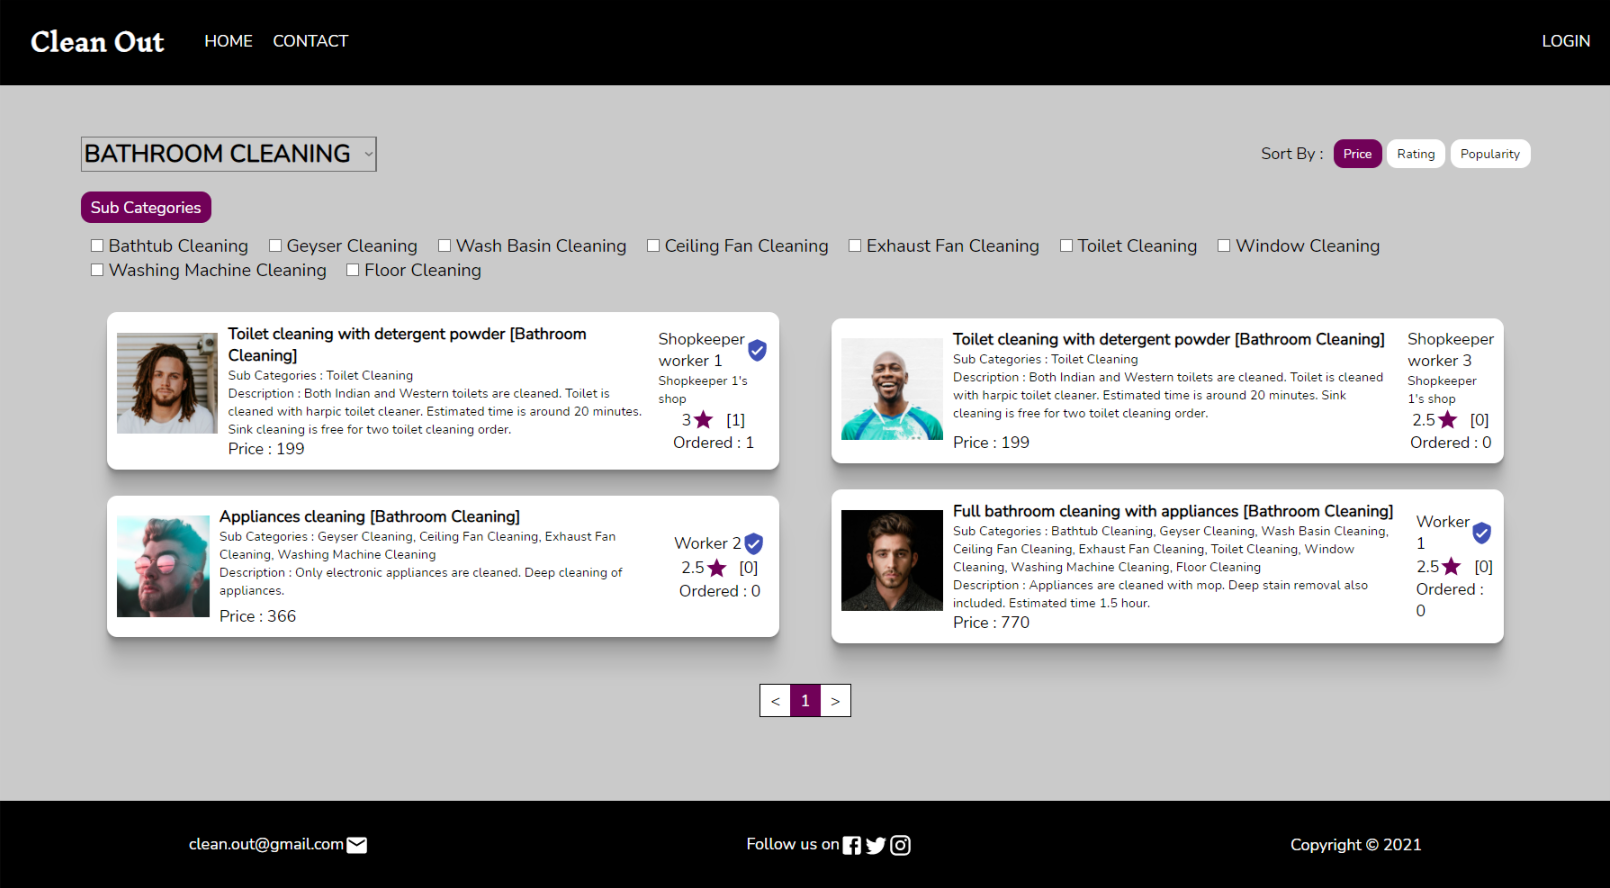
\includegraphics[width=8cm]{Testing pincode 2.png}
        \caption{Testing services based on pincode entered by customer}
        \label{fig:testPincode2}
    \end{figure}
    
    \item Each item and worker service has feedbacks. Feedback can be added and updated. We have tested addition and update in both of item and worker service. Below we have shown for worker service.
    \begin{figure}[H]
        \centering
        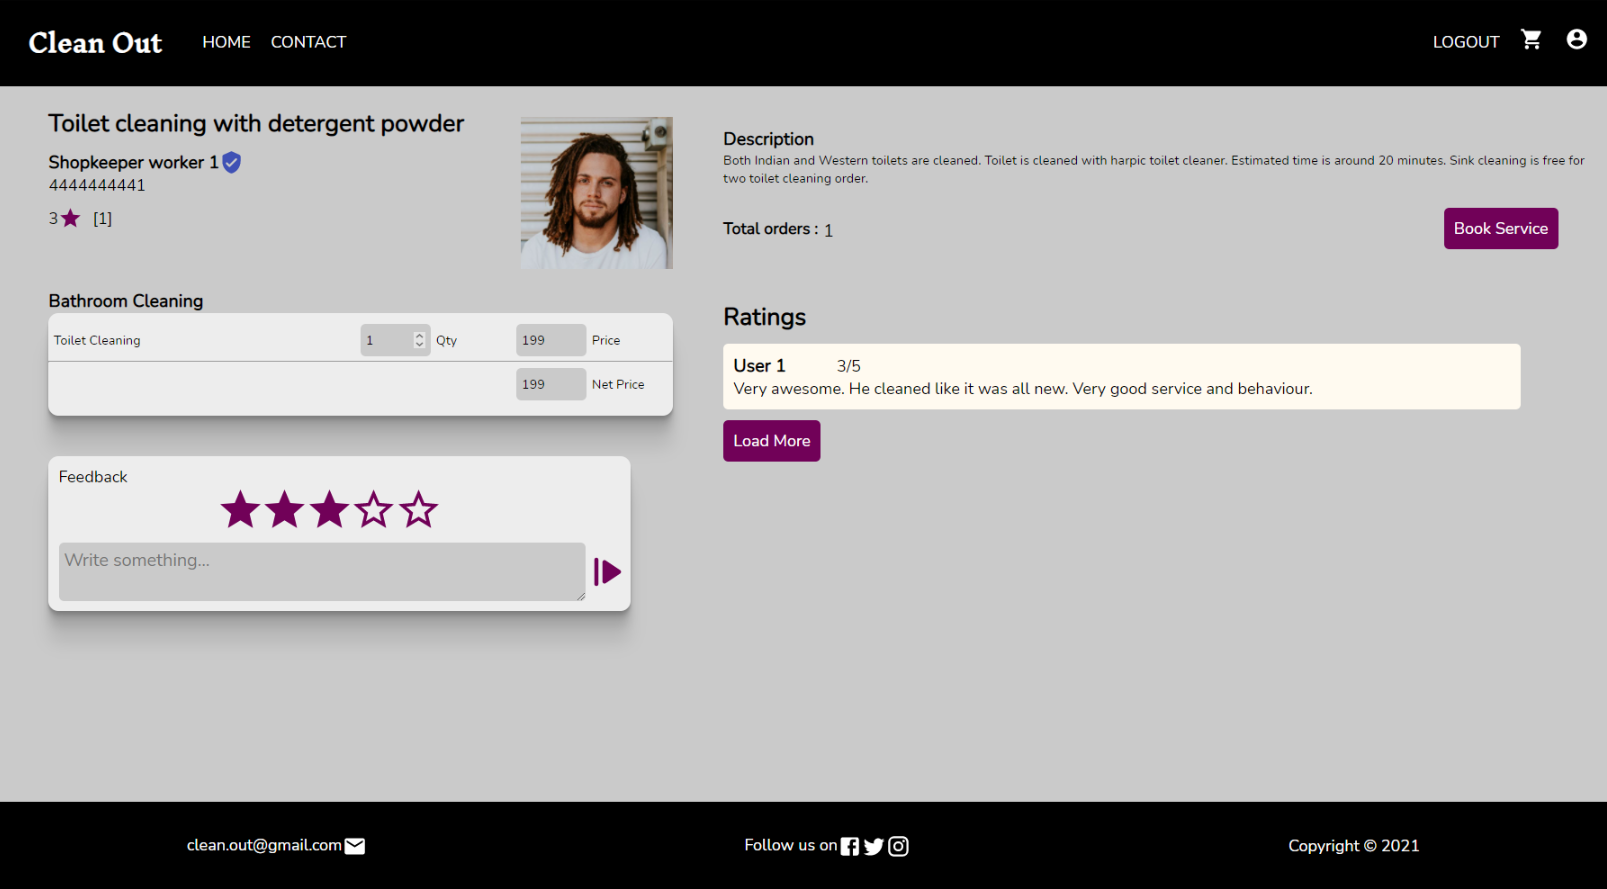
\includegraphics[width=8cm]{Testing feedback 1.png}
        \caption{Testing user 3's view before user 2 add feedback}
        \label{fig:testFeedback1}
    \end{figure}
    \begin{figure}[H]
        \centering
        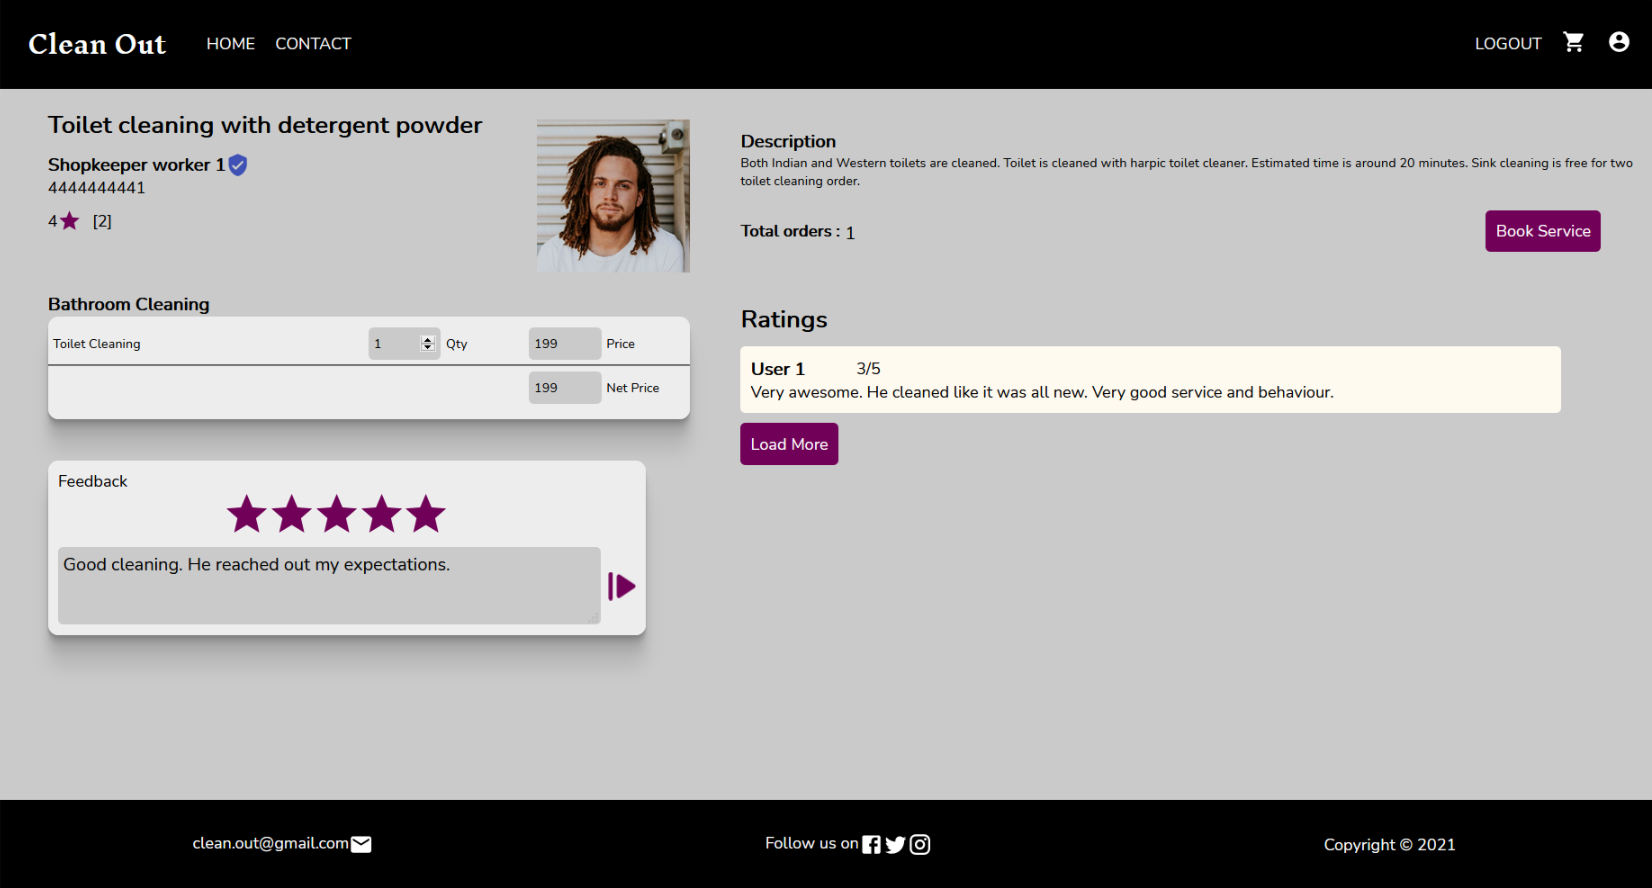
\includegraphics[width=8cm]{Testing feedback 2.png}
        \caption{Testing user 2 has added feedback}
        \label{fig:testFeedback2}
    \end{figure}
    \begin{figure}[H]
        \centering
        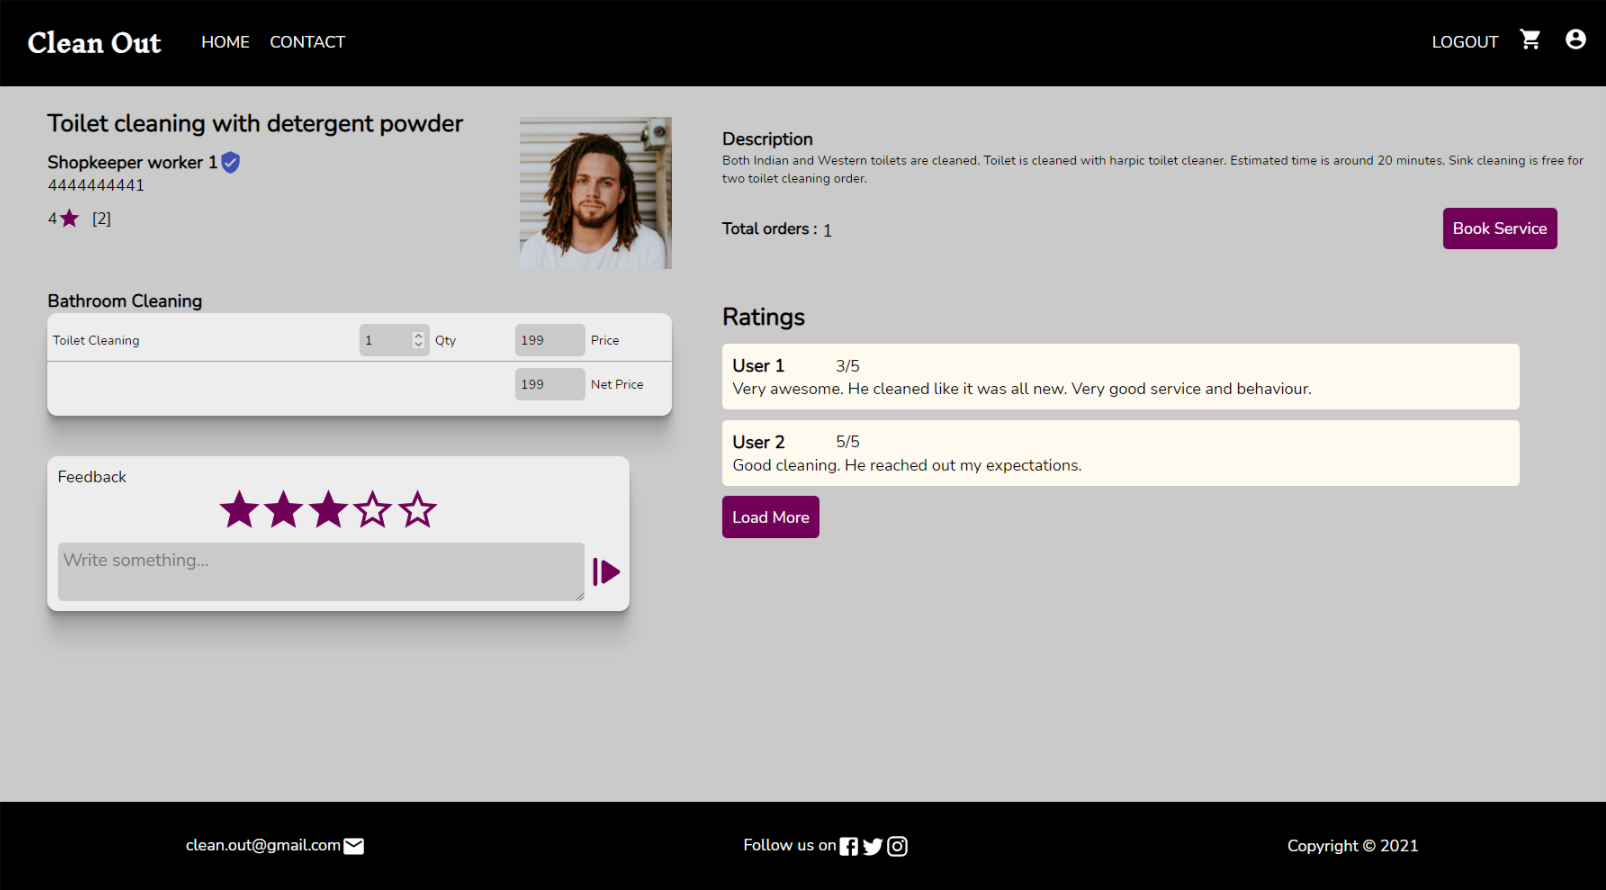
\includegraphics[width=8cm]{Testing feedback 3.png}
        \caption{Testing user 3's view after user 2 added feedback}
        \label{fig:testFeedback3}
    \end{figure}
    
    In figure \ref{fig:testFeedback1} we have shown the page when "user 3" is visiting the worker service. At this point "user 2" has not added feedback but "user 1" has already added feedback. In figure \ref{fig:testFeedback2} we have shown the page of "user 2" after "user 2" add feedback. Now in figure \ref{fig:testFeedback3} we have shown the view of "user 3" after the "user 2" add his feedback. We have tested this for cleaning item also and it is also giving correct results.
    
    \vspace{0.5cm}
    \item Then we have tested item order and service order feature. When customer place item order, customer himself and related all shopkeeper keeper should get service order notification and also they should be able to see the order in requested order field sort by latest date. Also when customer book service then customer and worker should get notification. If worker is not individual worker and serving under some shopkeeper then that shopkeeper should also get the notification. Both worker and shopkeeper should be able to see the latest placed order at the top of list of requested orders. \\
    
    Below we have shown requested orders page for both shopkeeper and its worker before customer book service.
    \begin{figure}[H]
        \centering
        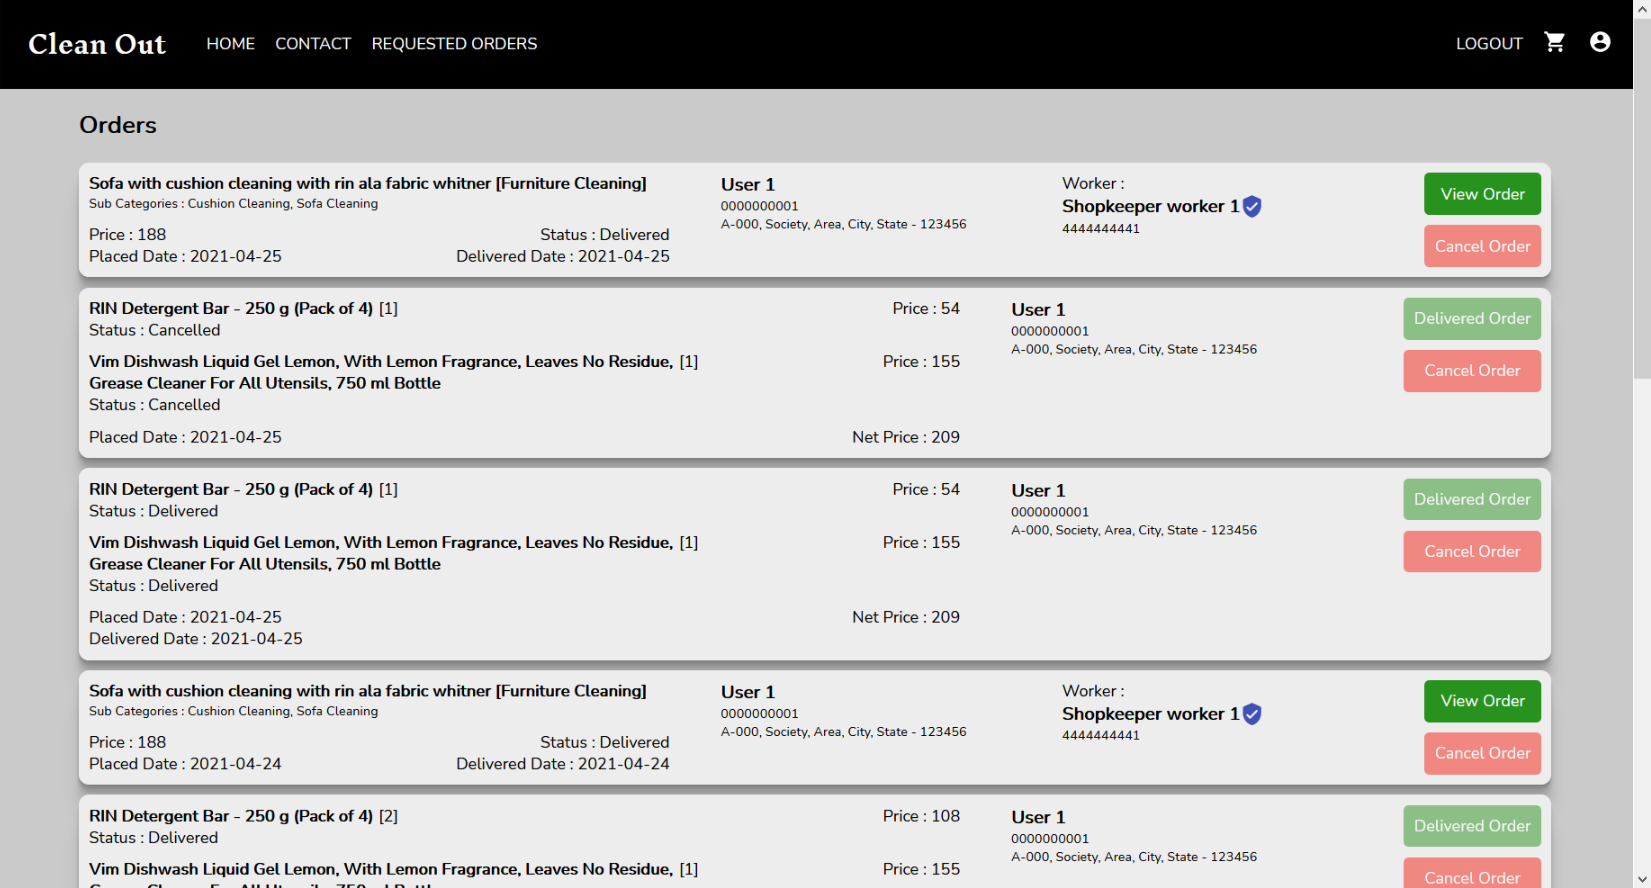
\includegraphics[width=8cm]{Testing service order shopkeeper.png}
        \caption{Testing requested orders page of shopkeeper before customer book service}
        \label{fig:testServiceOrderShopkeeper}
    \end{figure}
    \begin{figure}[H]
        \centering
        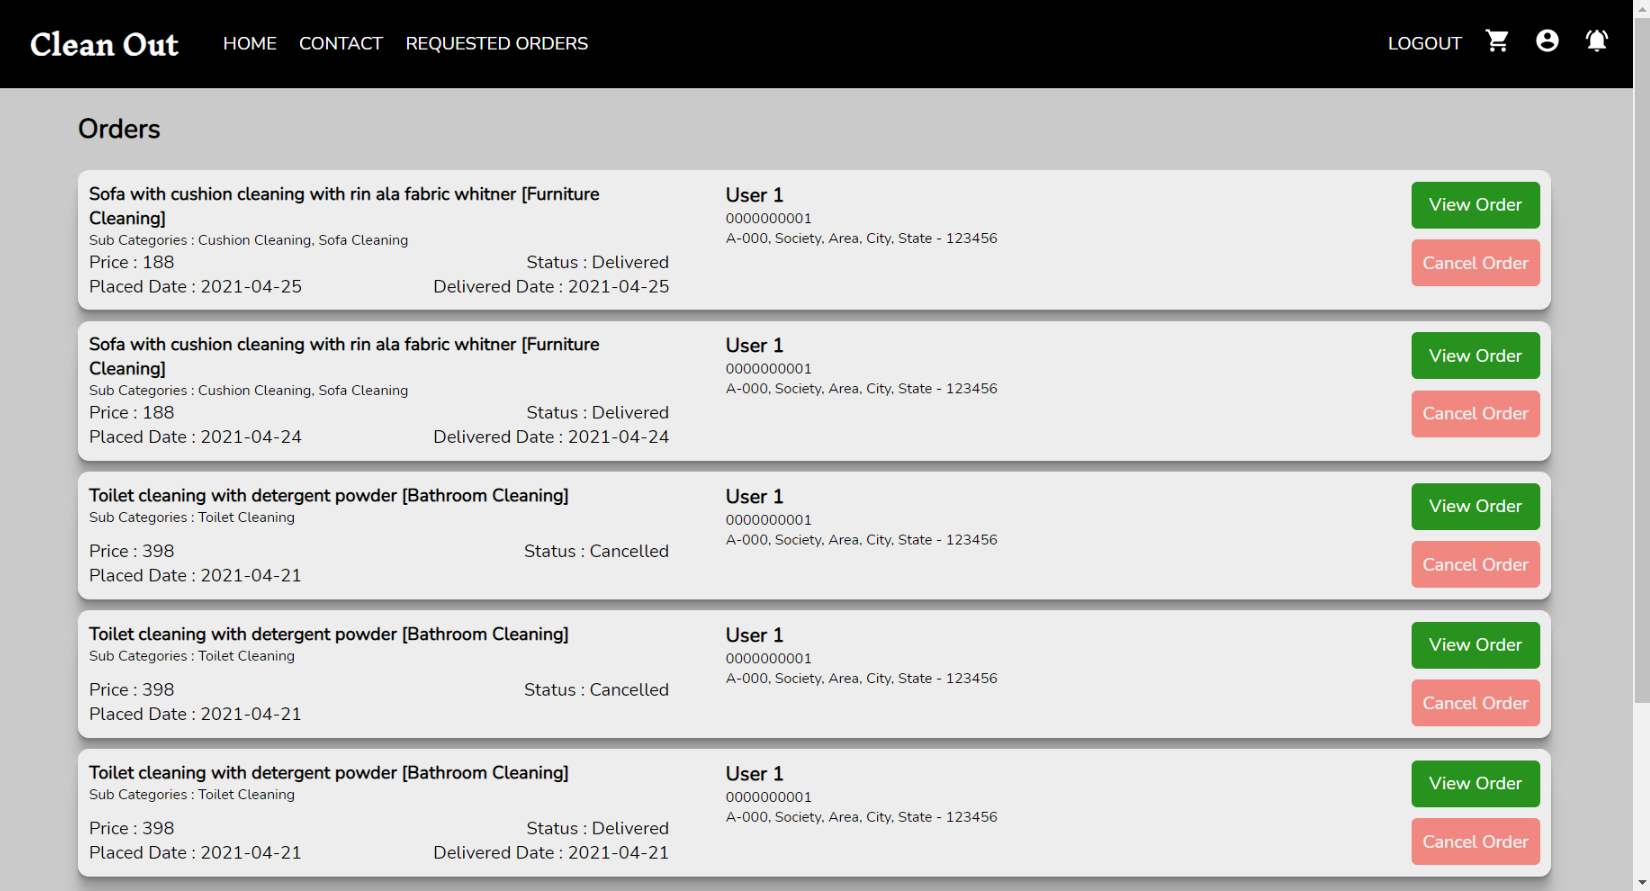
\includegraphics[width=8cm]{Testing service order worker.png}
        \caption{Testing requested orders page of worker before customer book service}
        \label{fig:testServiceOrderWorker}
    \end{figure}
    
    Now after customer booked the service that service order should be displayed at the top of the requested orders for both worker and shopkeeper. And customer also should be able to see their own order which is indeed the case which we have shown below. Here the customer name is "user 2".
    \begin{figure}[H]
        \centering
        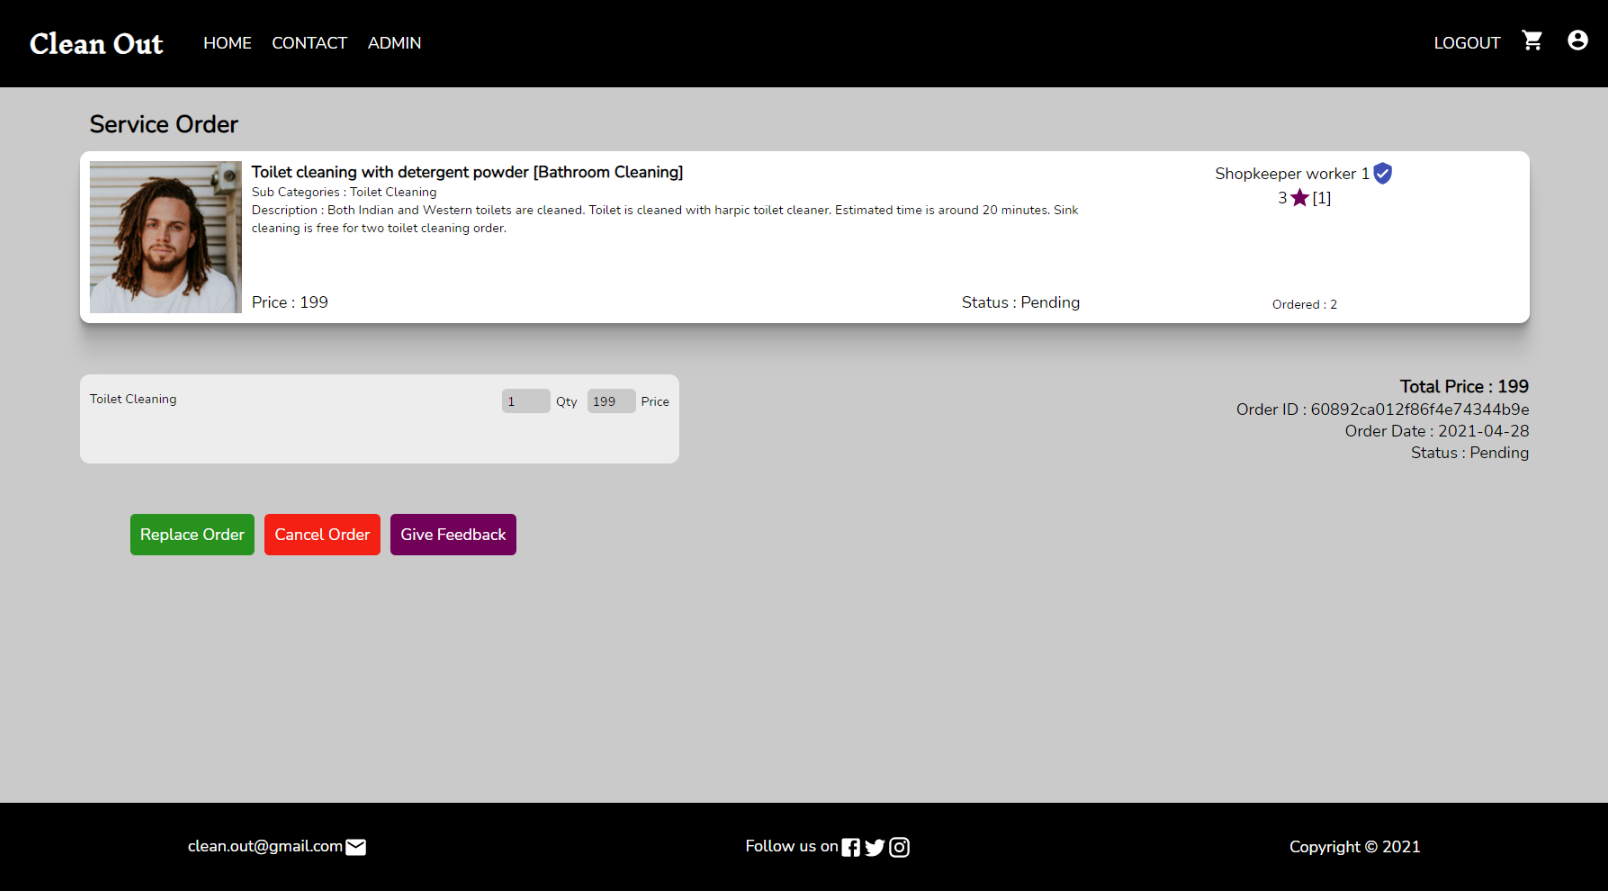
\includegraphics[width=8cm]{Testing service order user.png}
        \caption{Testing show service order to customer}
        \label{fig:testServiceOrderUser}
    \end{figure}
    \begin{figure}[H]
        \centering
        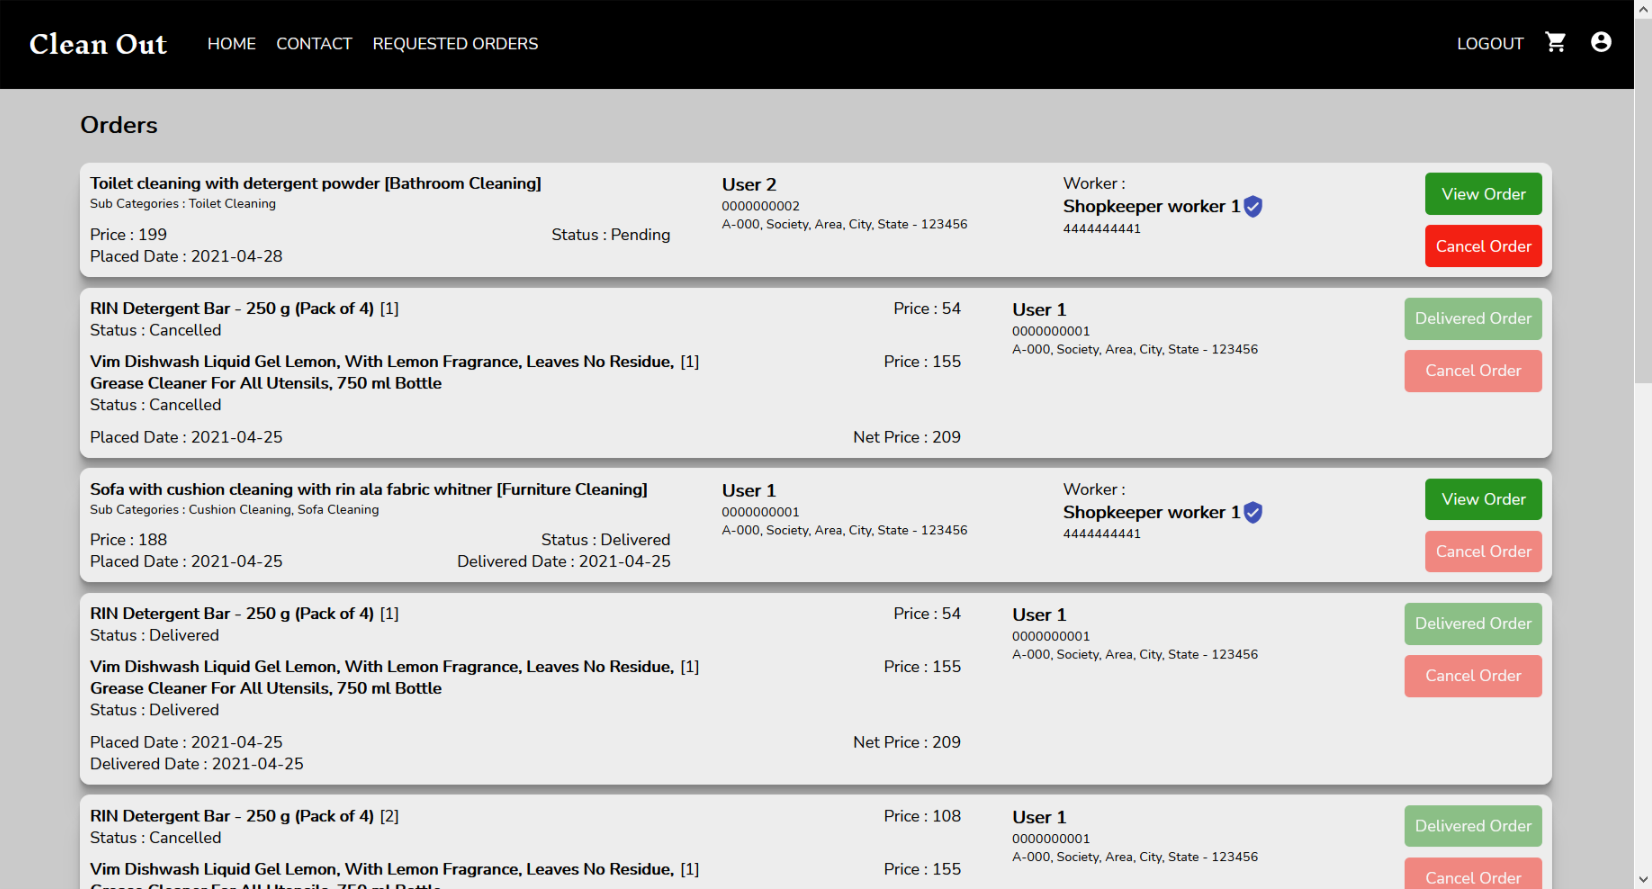
\includegraphics[width=8cm]{Testing service order shopkeeper 2.png}
        \caption{Testing show service order to shopkeeper}
        \label{fig:testServiceOrderShopkeeper2}
    \end{figure}
    \begin{figure}[H]
        \centering
        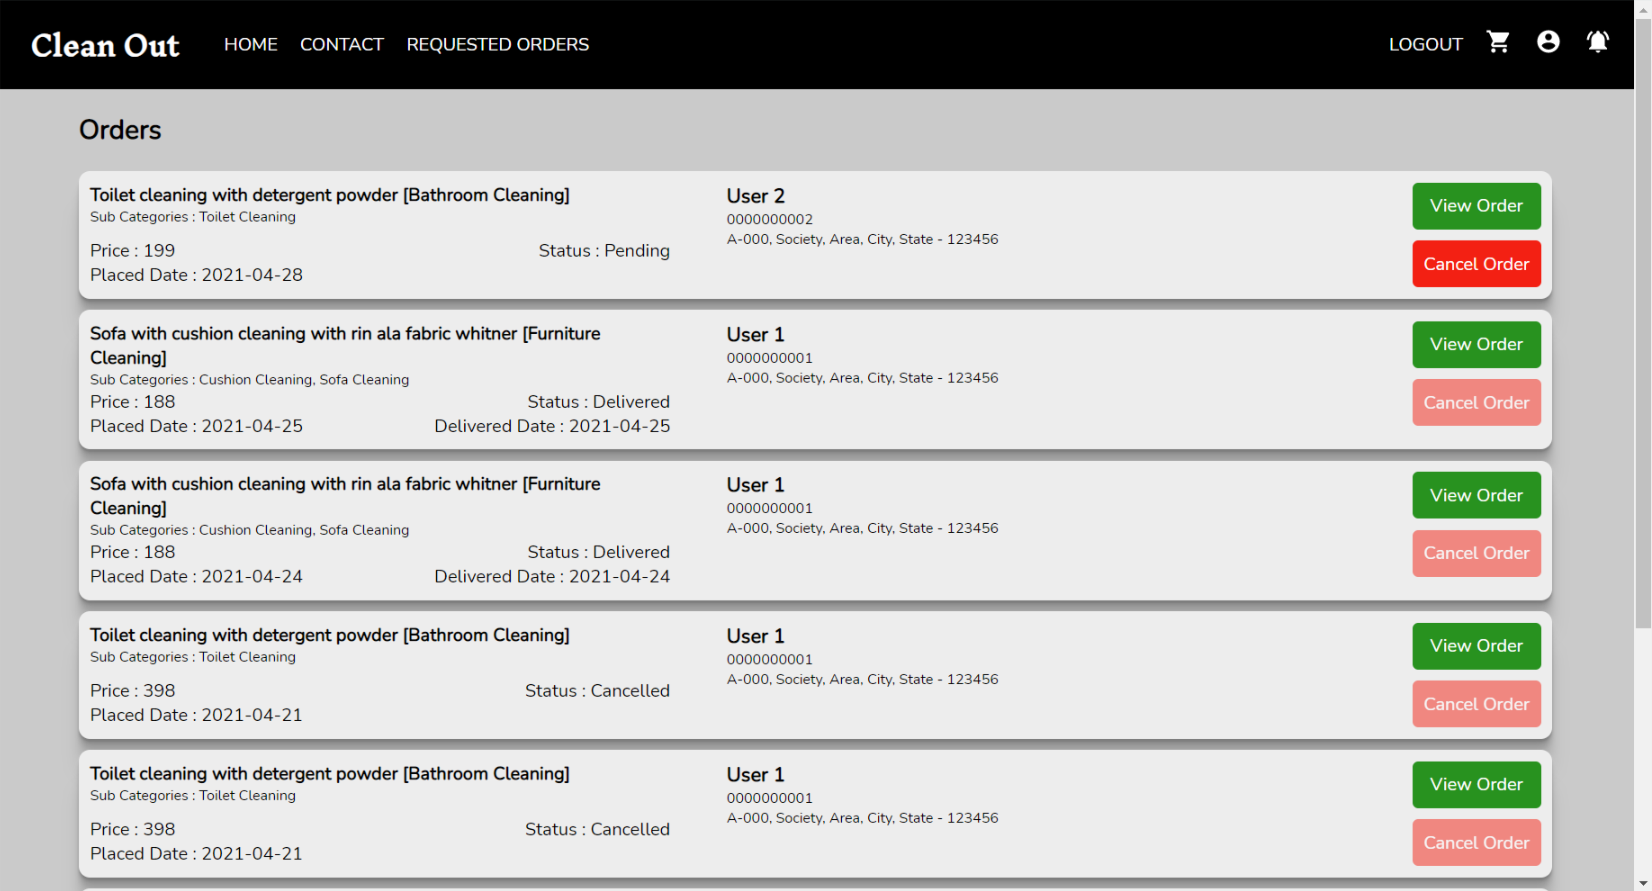
\includegraphics[width=8cm]{Testing service order worker 2.png}
        \caption{Testing show service order to worker}
        \label{fig:testServiceOrderWorker2}
    \end{figure}
    
    When the worker provides service completely then he goes to requested order and then open order and then click on done order. This will send notification to all the related parties. And also update the database which can be seen from blow figures. In between if due to any reason either worker or shopkeeper or customer cancel the order then also it changes database and sends notification to related parties. This is very similar to done order case so we have not shown result here but those test cases also passed. Similarly test cases for item order are also passed.
    \begin{figure}[H]
        \centering
        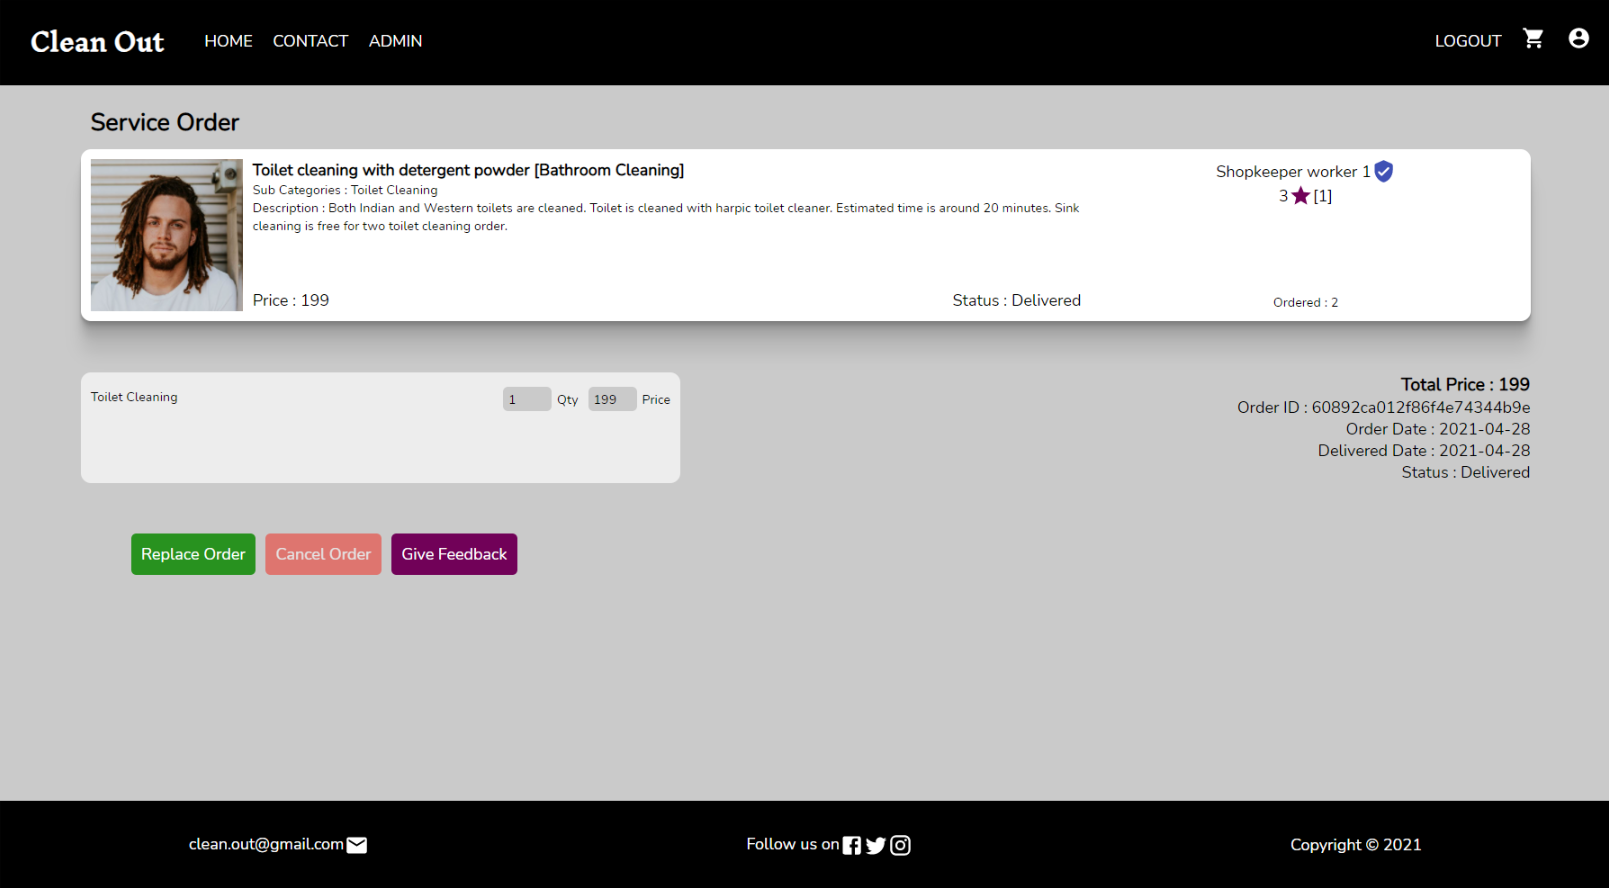
\includegraphics[width=8cm]{Testing service order user 2.png}
        \caption{Testing show service order to customer after order completion}
        \label{fig:testServiceOrderUser2}
    \end{figure}
    \begin{figure}[H]
        \centering
        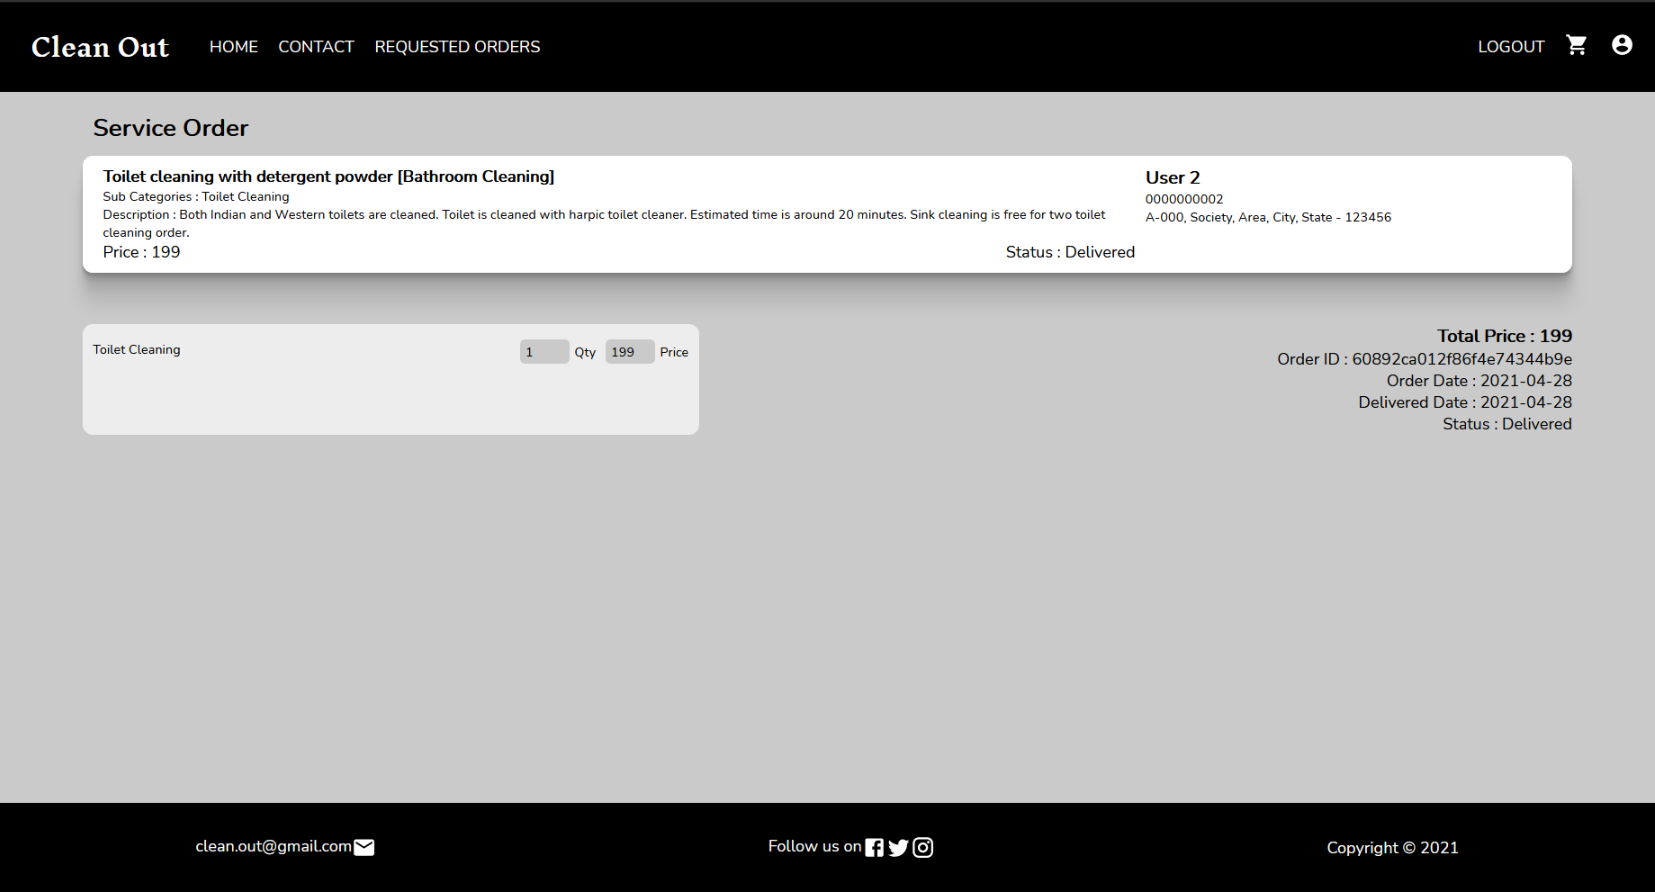
\includegraphics[width=8cm]{Testing service order shopkeeper 3.png}
        \caption{Testing show service order to worker and shopkeeper after order completion}
        \label{fig:testServiceOrderShopkeeper3}
    \end{figure}
    
    \item For admin there are many use cases but we focus mainly on find user, verify user and add/remove coadmin features. Admin/Coadmin can find user, worker or shopkeeper by phone number, pincode or user name. Which is giving correct result as shown below.
    \begin{figure}[H]
        \centering
        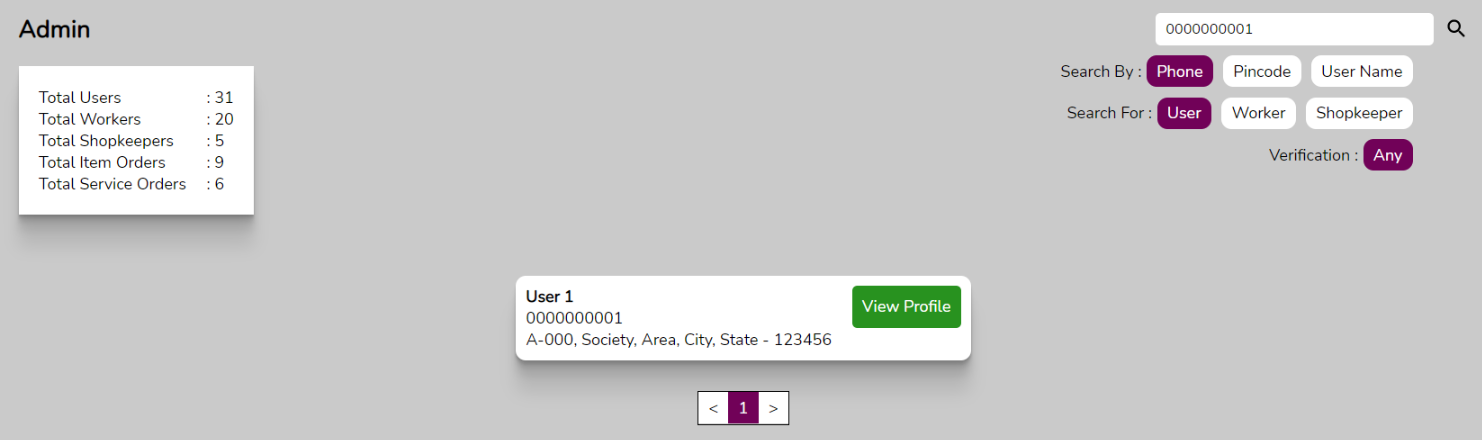
\includegraphics[width=8cm]{Testing admin phone.png}
        \caption{Testing show users search by phone}
        \label{fig:testAdminPhone}
    \end{figure}
    \begin{figure}[H]
        \centering
        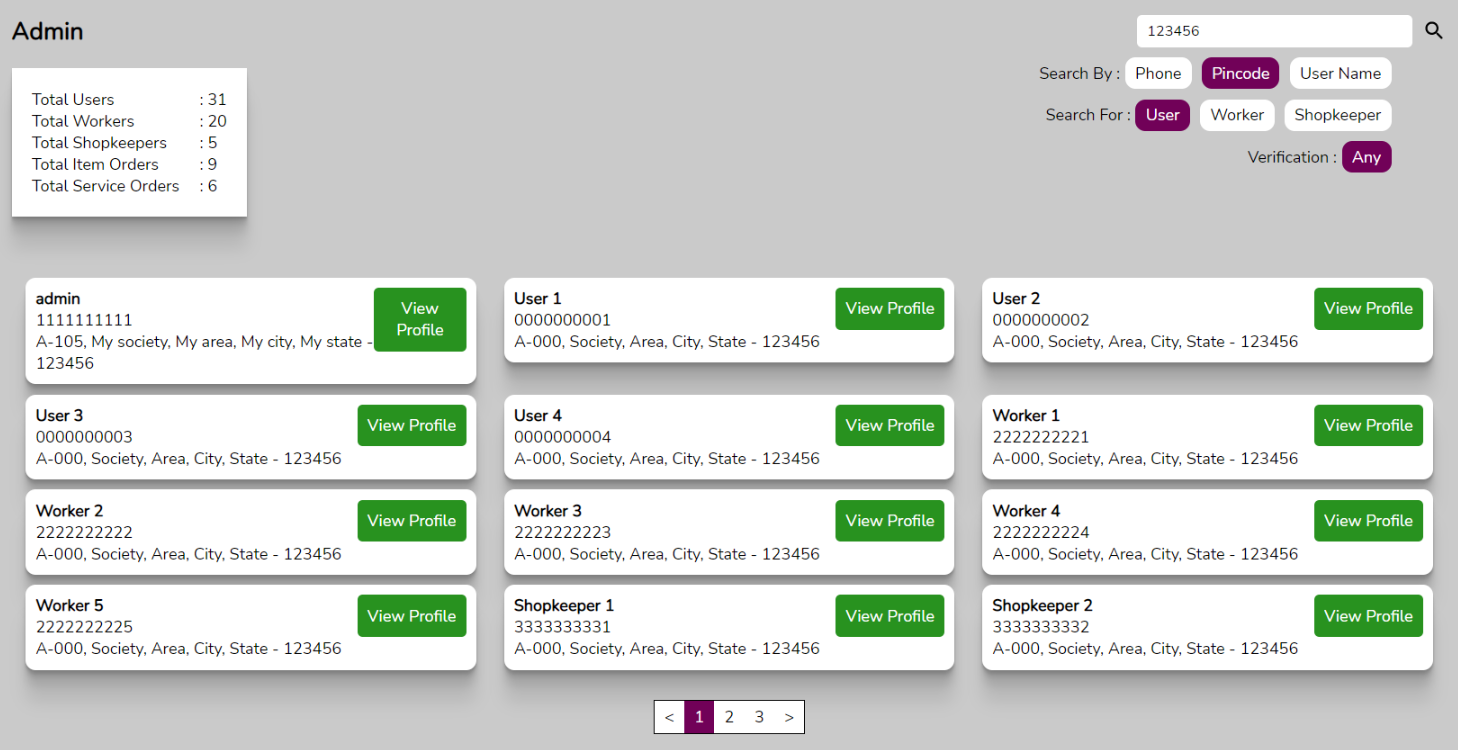
\includegraphics[width=8cm]{Testing admin pincode.png}
        \caption{Testing show users search by pincode}
        \label{fig:testAdminPincode}
    \end{figure}
    \begin{figure}[H]
        \centering
        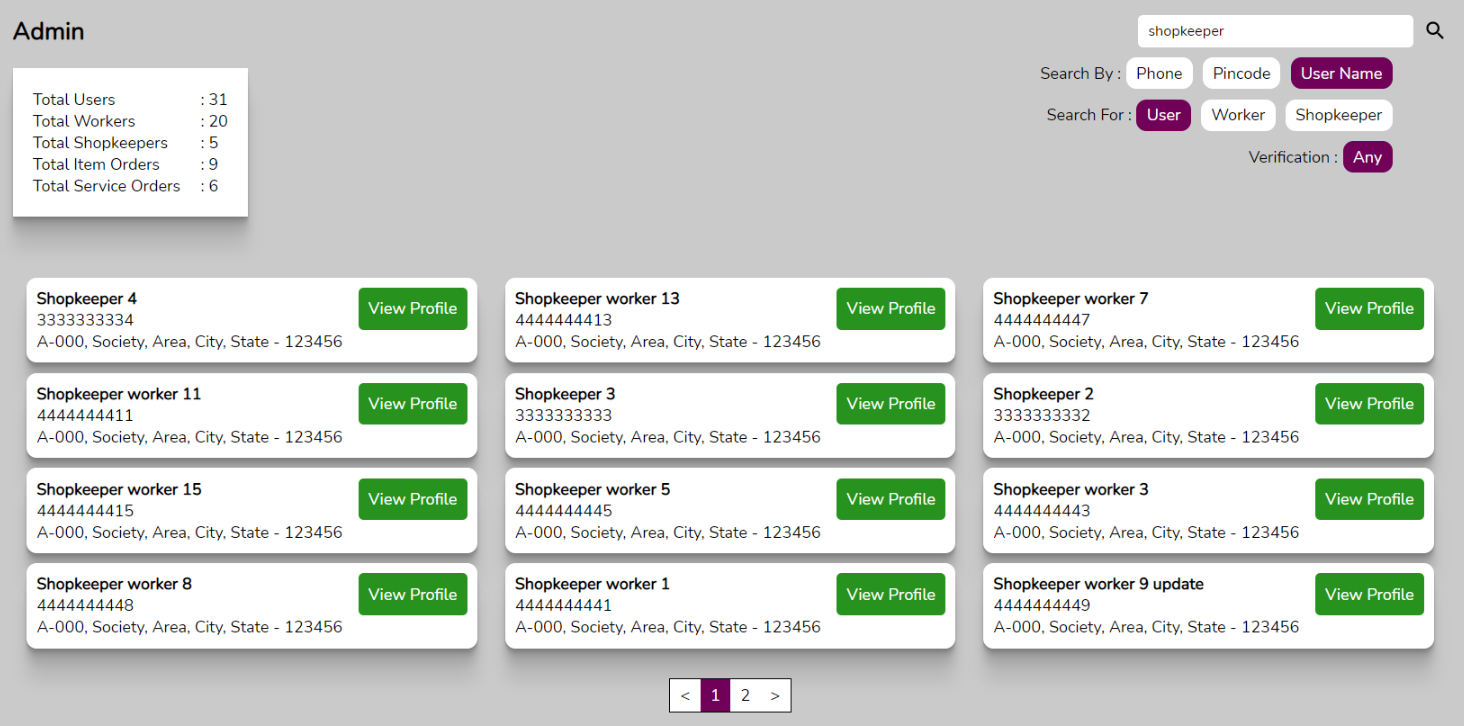
\includegraphics[width=8cm]{Testing admin username.png}
        \caption{Testing show users search by username}
        \label{fig:testAdminUsername}
    \end{figure}
    
    Then another thing is that admin/coadmin can verify worker or shopkeeper after viewing their proofs which is shown below.
    \begin{figure}[H]
        \centering
        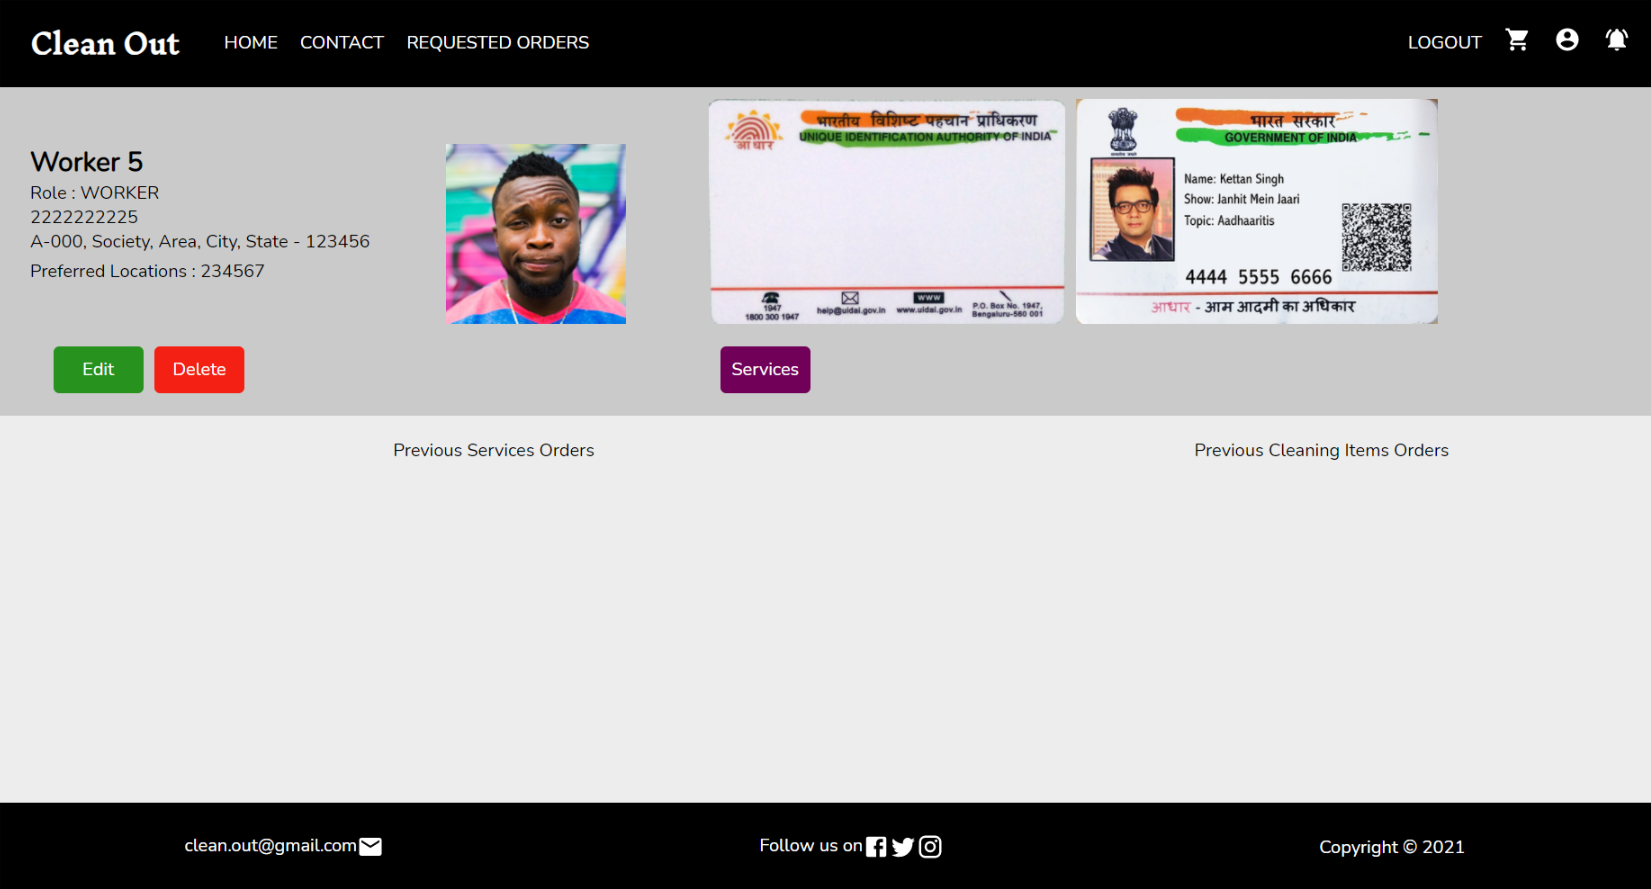
\includegraphics[width=8cm]{Testing admin verified before.png}
        \caption{Testing worker 5's profile before verification}
        \label{fig:testAdminVerifiedBefore}
    \end{figure}
    \begin{figure}[H]
        \centering
        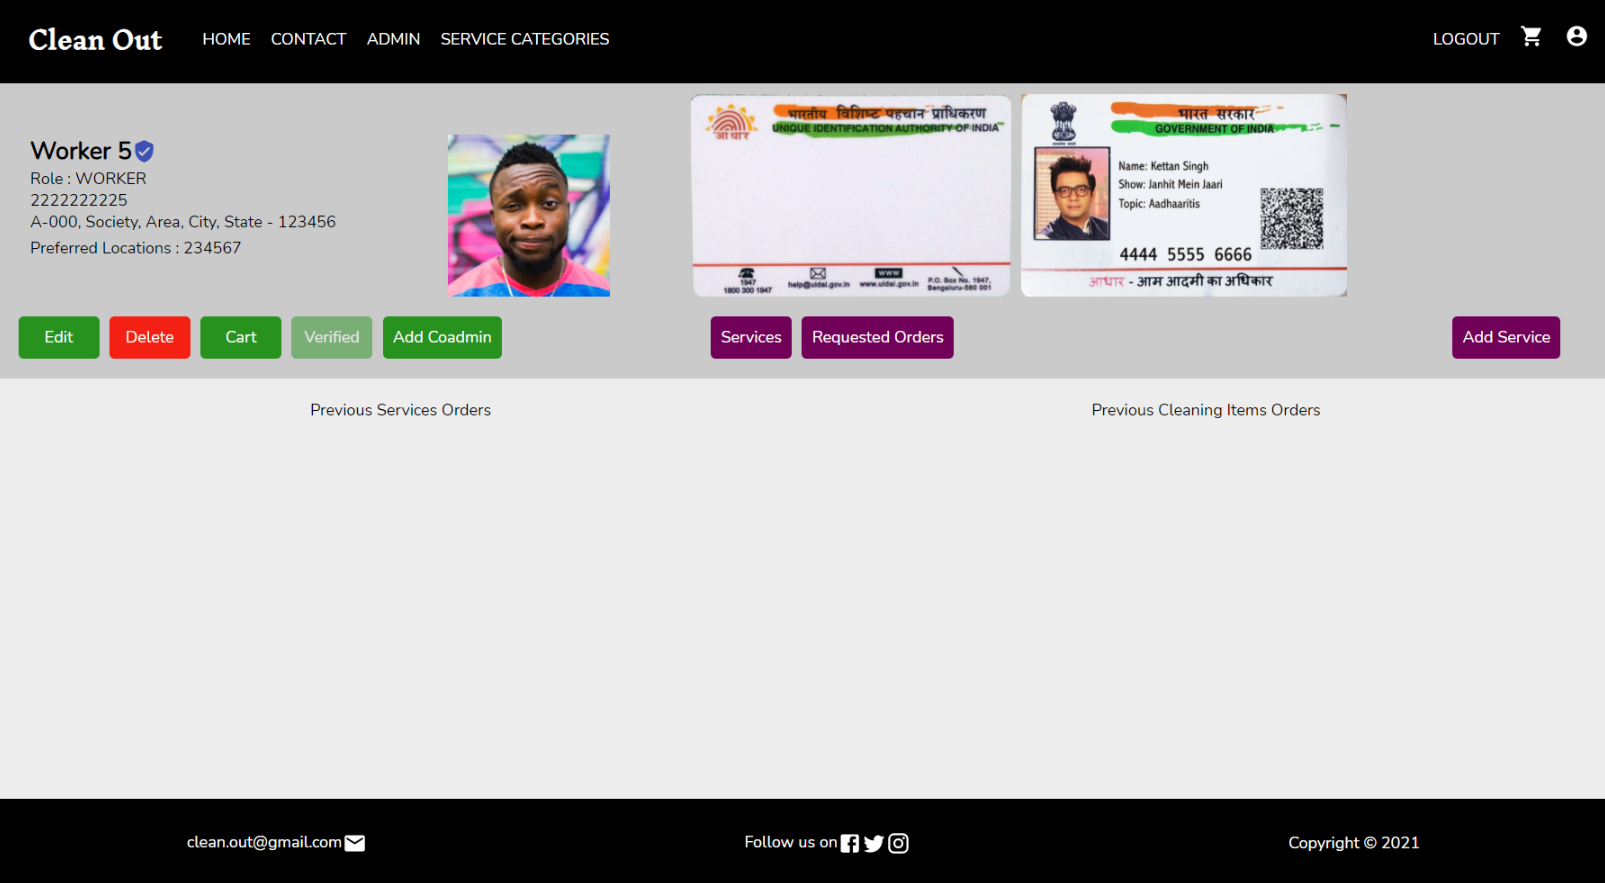
\includegraphics[width=8cm]{Testing admin verified during.png}
        \caption{Testing worker 5's profile in admin mode after admin clicked on verify button}
        \label{fig:testAdminVerifiedDuring}
    \end{figure}
    \begin{figure}[H]
        \centering
        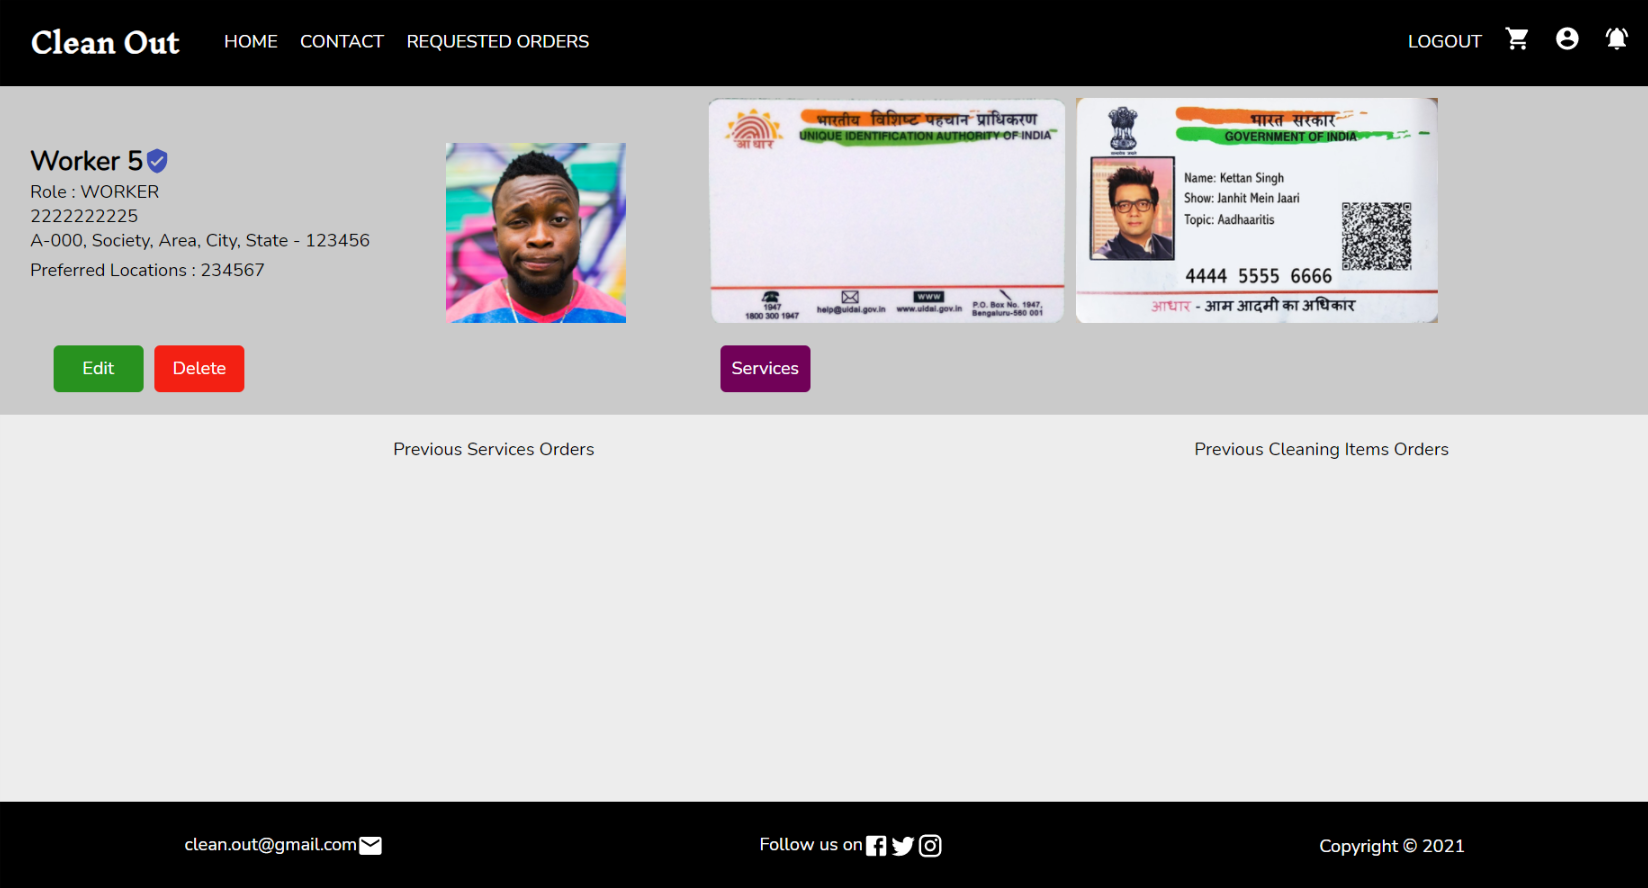
\includegraphics[width=8cm]{Testing admin verified after.png}
        \caption{Testing worker 5's profile after verification}
        \label{fig:testAdminVerifiedAfter}
    \end{figure}
    
    The next thing is to make a user coadmin. Removing coadmin is also same procedure so we have tested that but not shown here. Also a point to note is that the verify button shown in figure \ref{fig:testAdminVerifiedDuring} is shown only for admin user. It is hidden for user other than admin. So making coadmin and removing coadmin can only be done by admin. Which also we have tested but not shown here.
    \begin{figure}[H]
        \centering
        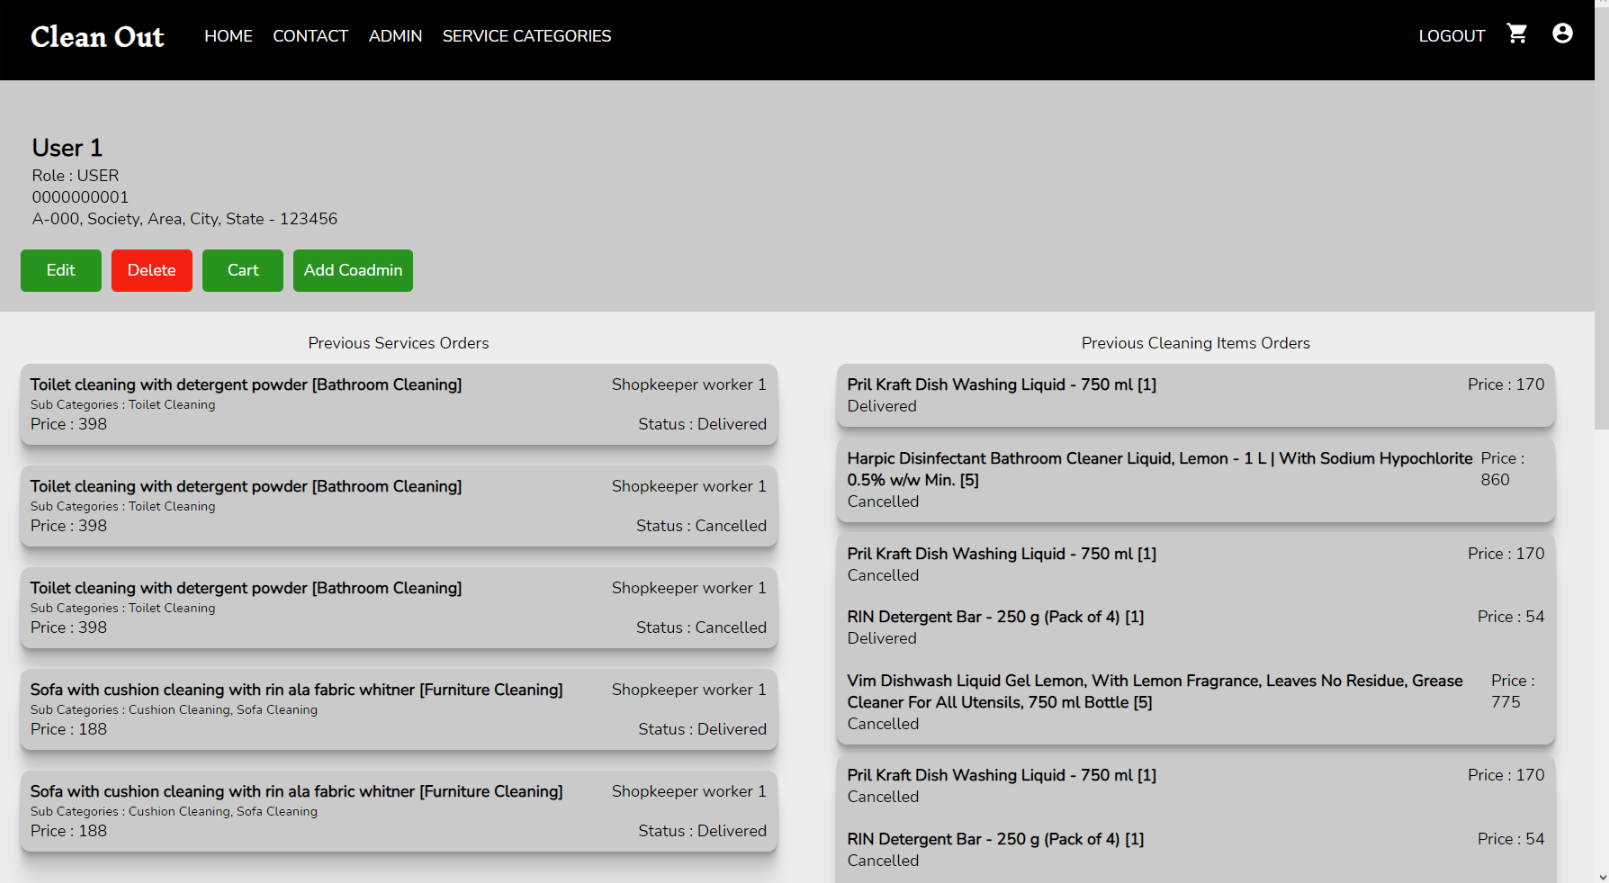
\includegraphics[width=8cm]{Testing add coadmin before.png}
        \caption{Testing user 1's profile before making coadmin for admin}
        \label{fig:testAddCoadminBefore}
    \end{figure}
    \begin{figure}[H]
        \centering
        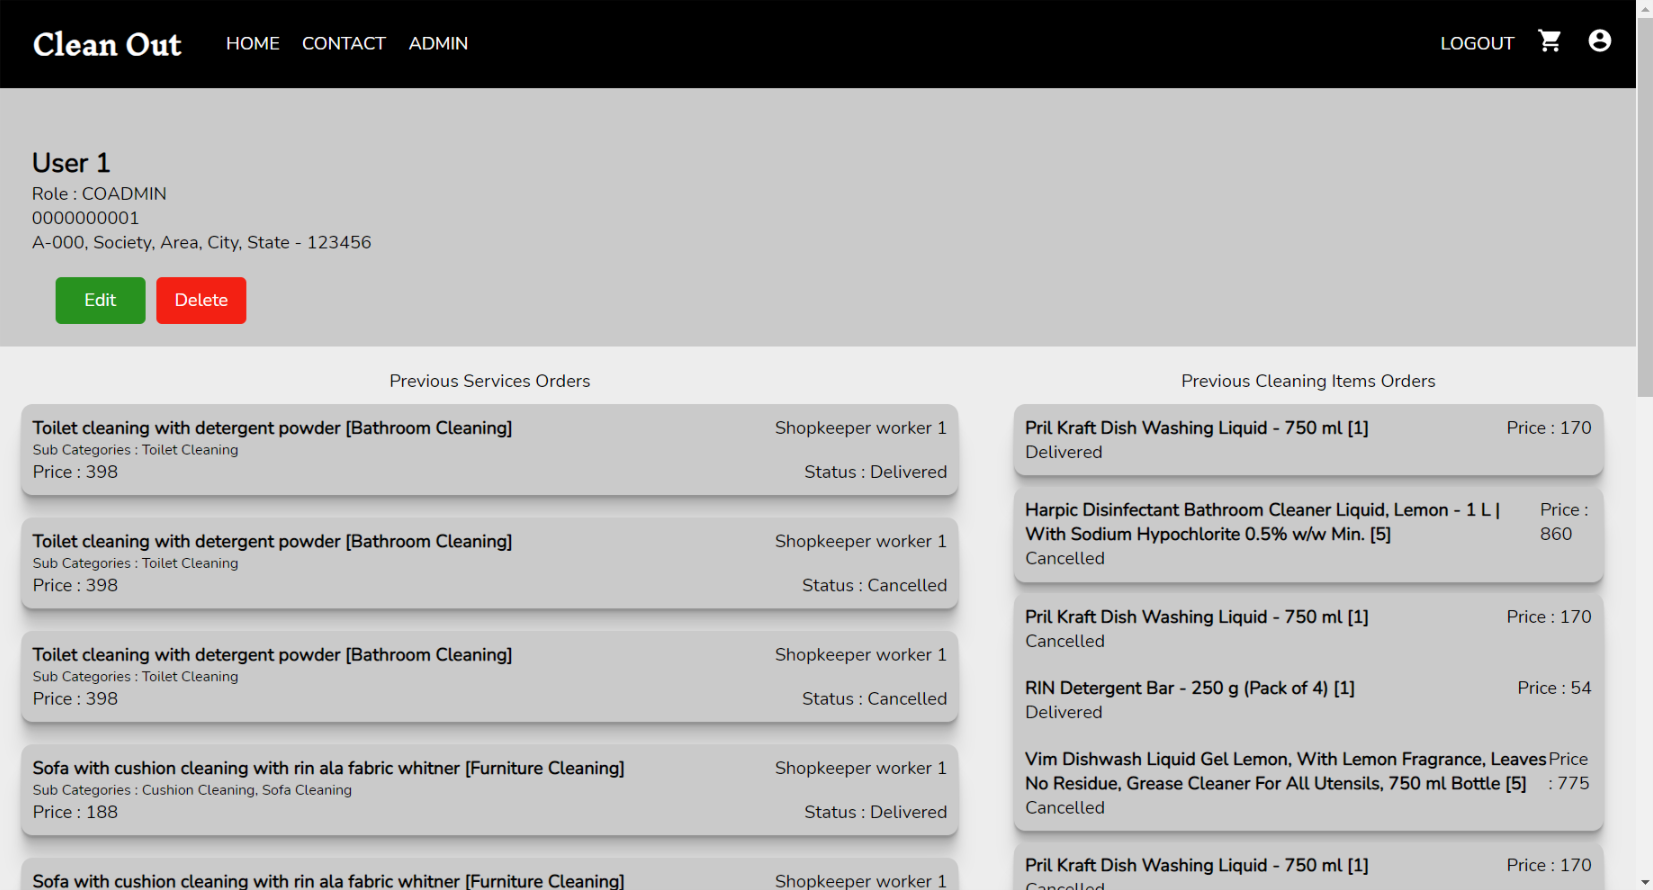
\includegraphics[width=8cm]{Testing add coadmin after.png}
        \caption{Testing user 1's profile after making coadmin for user 1}
        \label{fig:testAddCoadminAfter}
    \end{figure}
    
    
    
\end{itemize}





\vspace{1cm}
\section{Conclusion and Future work}
At this point the application is already robust and is quite efficient in terms of monitoring from Admin side. There is always a scope in improving the user interface. One can also add chat box feature in order to char directly between service provider and customer. Time scheduling feature can also be added where customer is asked to add preferred time slots at the time of booking service. Using AI user can be shown services based on previous data and also sent notification about it. Currently when user is not logged we ask manually to enter pincode of their area but it can be improved by automatically accessing location of user. Also in current application we have not used any external service which sends sms to registered phone numbers. Temporarily we have used nodemailer in the application which sends via email id but that just for testing purpose (you can see that in notification file of backend). The other thing is that right now we are sending notifications after exact one month of placed order to remind for the same order but it can be made more efficient and could be sent multiple notifications.






\vspace{1cm}
\section{Acknowledgement}
We would like to thanks Prof. Jayprakash Lalchandani from DAIICT, Gandhinagar, Gujarat, INDIA for giving us this opportunity and proper guidelines where possible. 

\end{document}